\chapter{FILTRAGEM F-K}
\label{cap3}

A transformada de Fourier (TF) constitui um dos maiores produtos da física e da matemática, e é indispensável na teoria e no processamento de sinais por várias razões. 
Uma das primeiras é que a sua base é estruturada no conceito de \textit{frequência}, o que permite uma compreensão melhor do fenômeno sendo estudado, e que adiciona um complemento ao sinal temporal (espacial) que é inicialmente usado para análise. 
Esta condição é muito comum, e os exemplos são vários na física de ondas (como na acústica, sísmica, eletromagnetismo, vibrações, ótica, etc.), bem como em outras áreas onde processos periódicos são importantes e regem os fenômenos de interesse (como na biomedicina, biologia, astronomia, economia, etc.). \cite{Lourenildo(2015)}

Para tornar a descrição mais prática, define-se o par das integrais direta, $G(\omega)$, e inversa, $g(t)$, em 1D nas seguintes formas ilimitadas (o que se faz para um lado $t,\omega \rightarrow +\infty$ se faz para o outro $t,\omega \rightarrow -\infty$):
\begin{equation}
G(\omega)=k_{1}\int_{-\infty}^{\infty}g(t)e^{-i\omega t}dt, \quad G(\omega)=F\{g(t)\}, \quad (i=\sqrt{-1}),
\label{eq.3.1}
\end{equation}
\begin{equation}
g(t)=k_{2}\int_{-\infty}^{\infty}G(\omega)e^{+i\omega t}d\omega, \quad g(t)=F^{-1}\{G(\omega)\}, \quad (\omega=2\pi f).
\label{eq.3.2}
\end{equation}
A escolha dos coeficientes $k_{1}$ e $k_{2}$ dependem do usuário ou do problema em estudo. O requerimento é que o produto $k_{1}k_{2}=1/2\pi$. Se $k_{1}=k_{2}$, então, $k_{1}=1/\sqrt{2\pi}$. Se $k_{1}=1$, então, $k_{2}=1/2\pi$.

Para o caso 2D, temos a TF direta na forma da equação (\ref{eq.3.3}) e TF inversa na equação (\ref{eq.3.4})

\begin{equation}
h(t, x)=\int_{-\infty}^{\infty} \int_{-\infty}^{\infty} H(f_{t}, f_{x}) e^{+i 2 \pi(f_{t} t+f_{x} x)} df_{t} df_{x}
\label{eq.3.3}
\end{equation}
\begin{equation}
H(f_{t}, f_{x})=\int_{-\infty}^{\infty} \int_{-\infty}^{\infty} h(t, x) e^{-i 2 \pi(f_{t} t+f_{x} x)} dt dx
\label{eq.3.4}
\end{equation}

Para estas equações se tem as relações: $f_{t}=\frac{1}{T} $, $f_{x}=\frac{1}{\lambda}=\frac{1}{vT}$, de onde se estabelece a relação $f_{t}=vf_{x}$; isto é, nestas condições a frequência temporal, $f_{t}$, e a frequência espacial, $f_{x}$, são acopladas através de uma relação linear $f_{t}=vf_{x}$, onde $v$ é o parâmetro de inclinação.
Também, usando a vagarosidade $s=\frac{1}{v}$ se tem a forma $f_{x}=sf_{t}$. 
A figura \ref{fig:Relacao_Dispersao} mostra a relação entre estas quantidades, com a descrição da propagação de uma onda plana, e a relação denominada de dispersão que envolve as frequências espaciais e a temporal.

\begin{figure}[H]
\centering
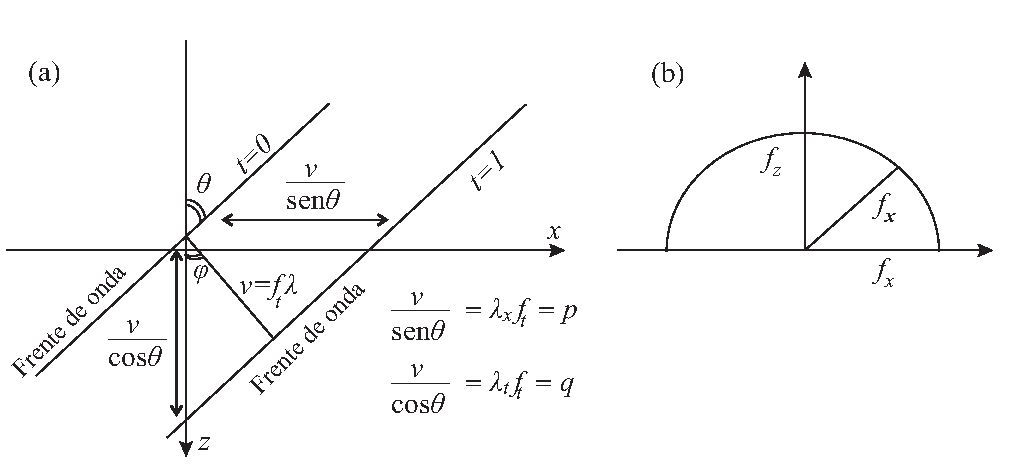
\includegraphics[width=12cm]{figuras/cap3/Relacao_Dispersao.pdf}
\vspace{-0.3cm}
\caption{Descrição física da relação entre a frente de onda e a equação da dispersão. 
(a) Propagação da onda plana. 
(b) Relação entre as componentes $f_{x}$ e $f_{z}$ e a total $f_{\mathbf{x}}$ para $f_{t}$ constante.}
\label{fig:Relacao_Dispersao}
\end{figure}

\section{Filtros de corte na frequência}

O princípio a ser aplicado é o de que os eventos possam ser separados no domínio da frequência, $f_{t}-f_{\mathbf{x}}$, de alguma forma, pelo menos parcial.  
Partindo deste princípio, a figura \ref{fig:Analise_Idealizada_Sinal_Ruido_Frequencia} ilustra a composição espectral, e serve para a análise da relação frequência temporal-espacial (número de onda) do conteúdo de velocidades comumente presente em experimentos de sísmica de exploração.

\begin{figure}[H]
\centering
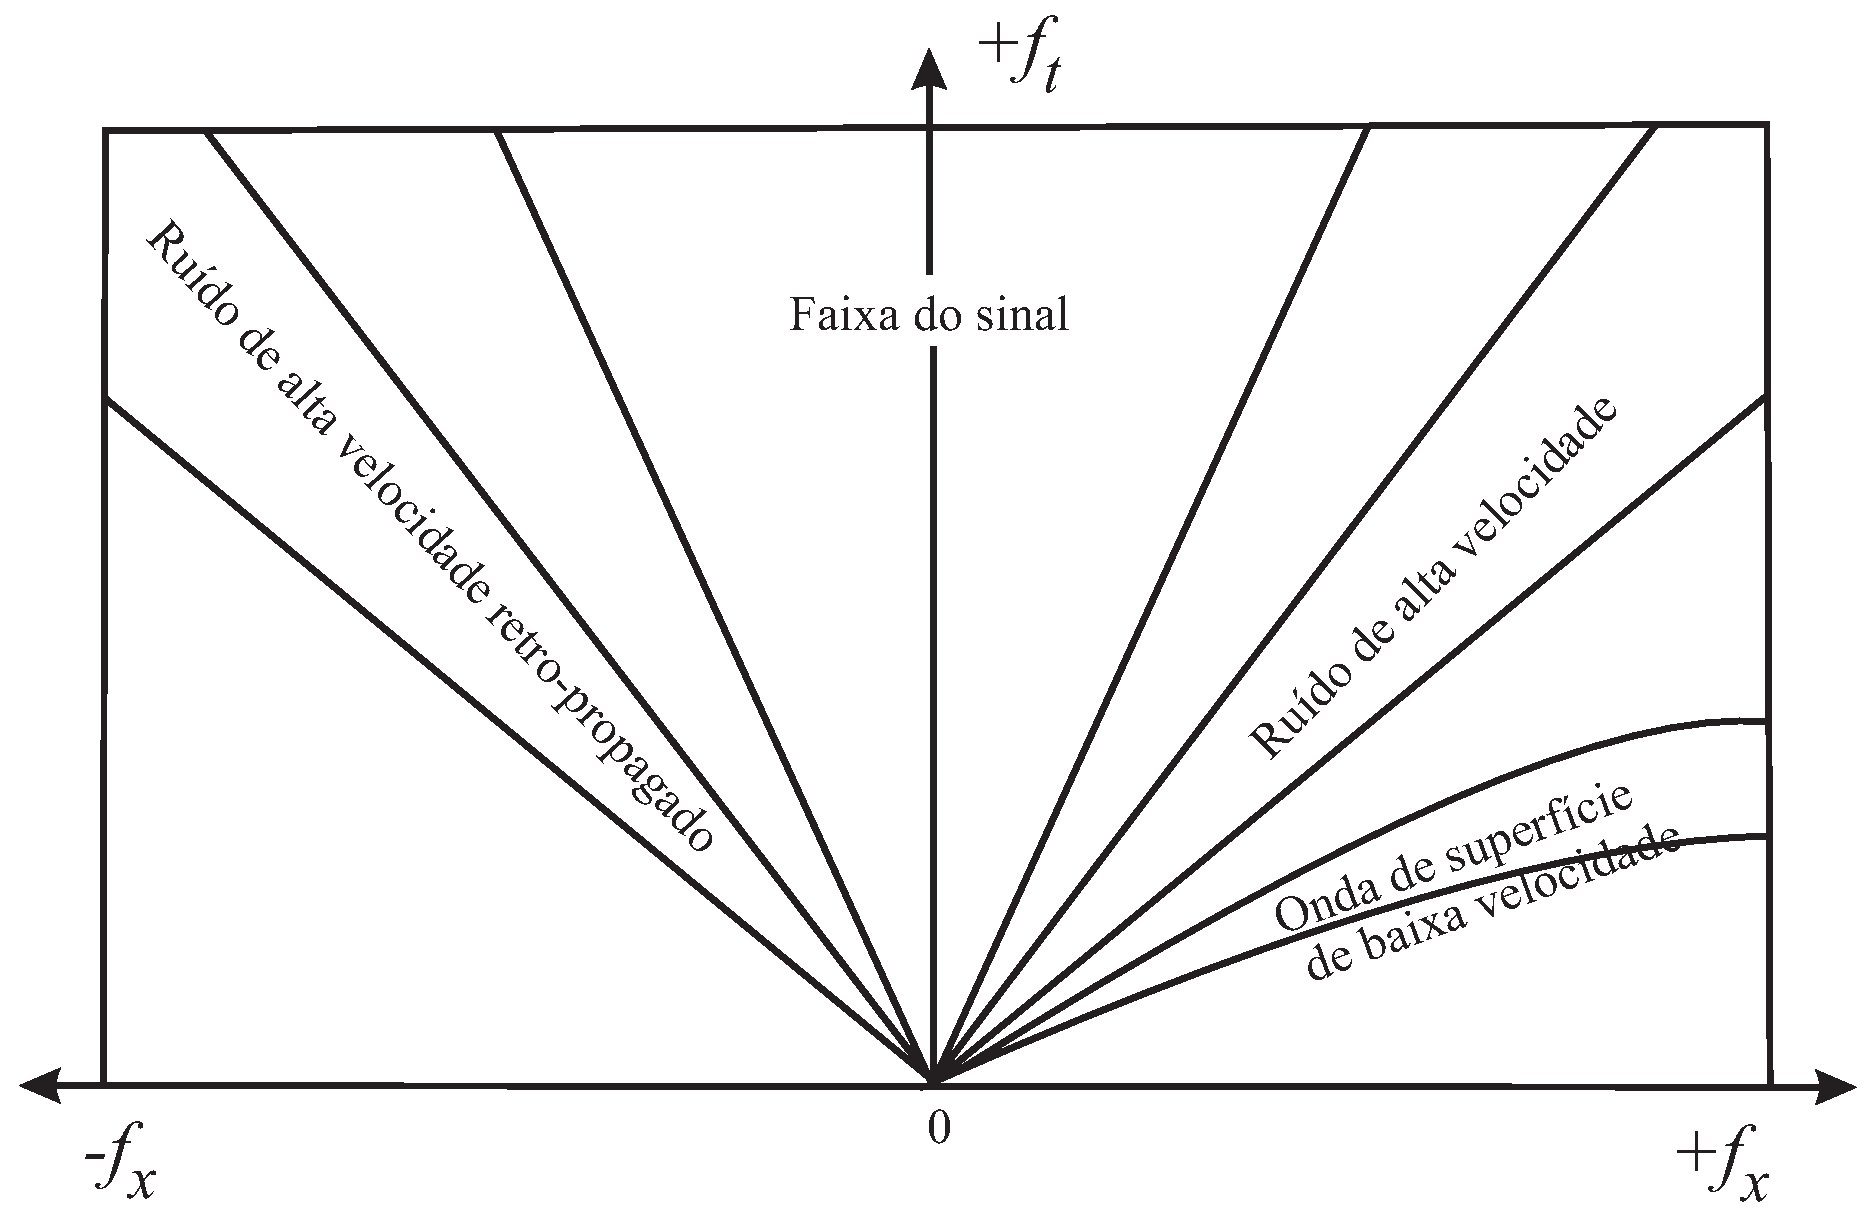
\includegraphics[width=11cm]{figuras/cap3/Analise_Idealizada_Sinal_Ruido_Frequencia.pdf}
\vspace{-0.3cm}
\caption{Ilustração da composição espectral de uma seção sísmica (frequência temporal-espacial). 
Se destacam as linhas de sinal de informação, ruídos de velocidade alta e baixa, e ruido das ondas de superfície de baixa frequência. As linhas inclinadas separam os eventos mergulhantes no domínio $f_{t}-f_{\mathbf{x}}$.}
\label{fig:Analise_Idealizada_Sinal_Ruido_Frequencia}
\end{figure}

A figura \ref{fig:Analise_Idealizada_Filtro_Separa} ilustra o problema que se encontra na tentativa de se aplicar um filtro, $H(f_{t},f_{x})$, convencional simples, o que se ilustra com a figura \ref{fig:Filtro_velocidade}, que tem por finalidade esboçar a relação linear simples (outra forma qualquer pode ser desenhada) no domínio espectral para o caso prático de dados no domínio do discretizado; as frequências de Nyquist estão definidas: 
$f_{Nt}=\frac{1}{2 \Delta t}$, $f_{Nx}=\frac{1}{2 \Delta x}$ e $f_{Nt}= vf_{Nx} =\frac{v}{2 \Delta x}$.
Neste caso, $v$ é a velocidade e $s$ é a vagarosidade.
Observe-se na figura \ref{fig:Filtro_velocidade} as faixas de passagem e de rejeição lineares, onde está superposto uma ilustração de uma linha de contorno típica (forma qualquer) do espectro de um dado real. 
A relação entre as linhas de corte (passagem-rejeição) linear e espectro real não é simples, o que se deseja é que as linha sejam o mais alinhado (paralelo) possível.
%=====================================================
\begin{figure}[H]
\centering
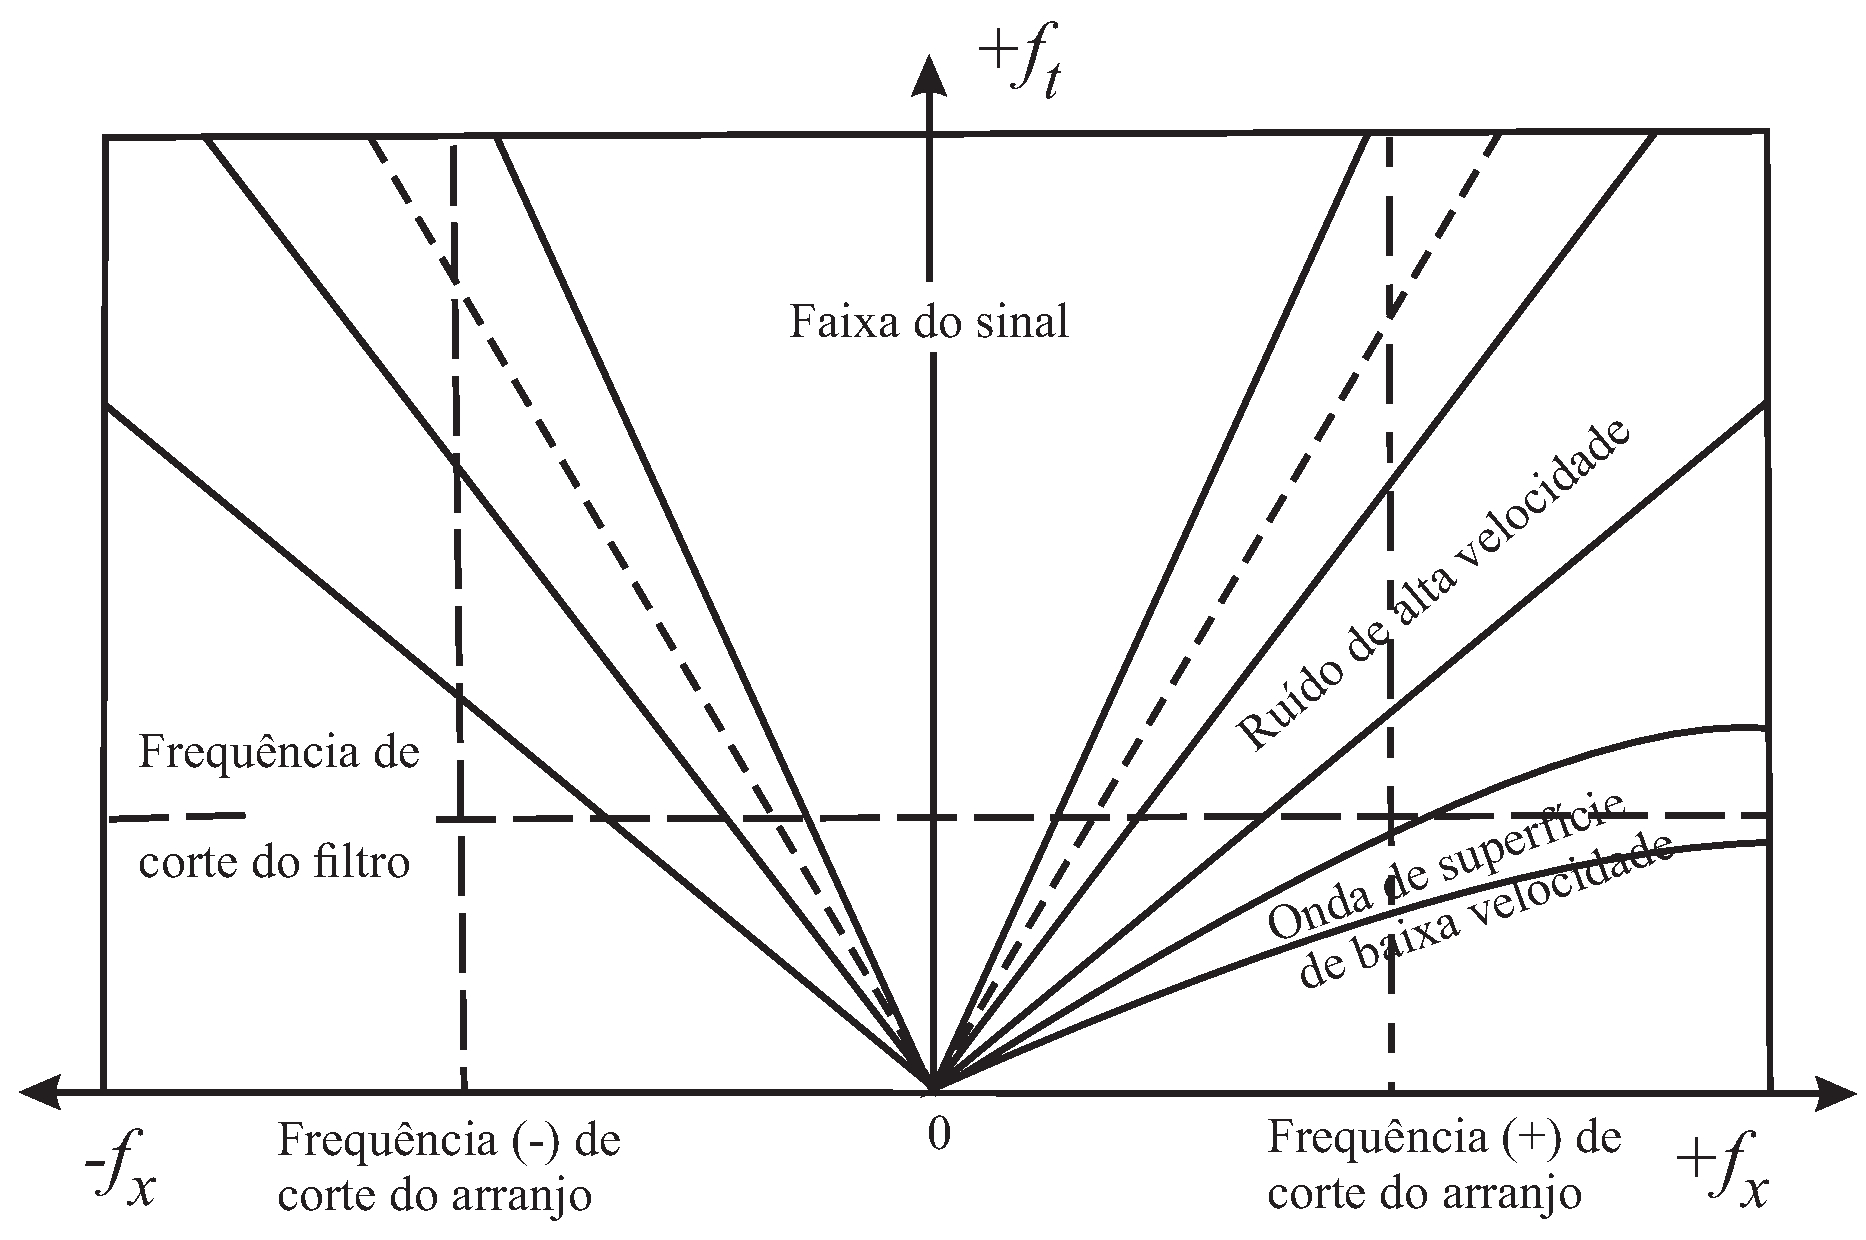
\includegraphics[width=11cm]{figuras/cap3/Analise_Idealizada_Filtro_Separa.pdf}
\vspace{-0.3cm}
\caption{Construção idealizada do filtro para separação da composição espectral de uma seção sísmica (frequência temporal-espacial) correspondente à figura \ref{fig:Analise_Idealizada_Sinal_Ruido_Frequencia}. 
Se destacam as linhas de sinal de informação, ruídos de velocidade alta e baixa, e ruido das ondas de superfície de baixa frequência.}
\label{fig:Analise_Idealizada_Filtro_Separa}
\end{figure}
%=====================================================
%=======================================================
\begin{figure}[H]
\centering
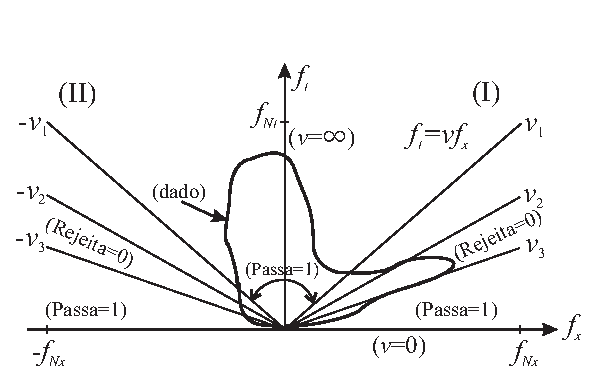
\includegraphics[width=12cm]{figuras/cap3/Filtro_velocidade.pdf}
\vspace{-0.3cm}
\caption{Divisão do domínio da frequência 2D em quadrantes, ilustração do espectro de (dado) real, $H_{R}(f_{t},f_{x})$, e desenho do filtro com a forma Em-leque de Passagem-Rejeição (EL-P-R). 
Para completar o filtro é necessário refletir os quadrantes: I para III e II para IV.}
\label{fig:Filtro_velocidade}
\end{figure}
%=======================================================

A figura \ref{fig:Analise_Idealizada_Filtro_Separa} esboça a tentativa de se preservar uma banda de frequências mais ampla possível. 
Para isto se analisa a geometria do arranjo de registro (padrão de distribuição dos sensores nas estações, padrão de tiro, etc.), e ao passo que as dimensões geométricas do arranjo aumenta, a linha de corte vai no sentido de $f_{x}$ menor (comprimento de onda maior). 
Ao passo que as dimensões do arranjo aumenta, o sistema atenua a informação de eventos de mergulho (linear) e ruído.
E se as dimensões continuam aumentando, o corte passa para o leque do sinal de informação (Faixa do sinal).

\section{FILTRAGEM F-K DA SEÇÃO TIRO 50}

Após a aquisição do dado sísmico figura (\ref{fig:afastamento_min}) no $SU$ com a subrotina \textit{triseis} utilizou-se o tiro $50$ para a filtragem F-K no \textit{matlab}, onde foi implementado os plots da seção tiro figuras (\ref{fig:tiro_50}), (\ref{fig:tiro_50gain}), (\ref{fig:tiro_50ruido}) e (\ref{fig:tiro_50ruido_gain}). 

O ruído é intrínseco ao registro do traço sísmico, seja como consequência do meio geológico ou do próprio equipamento de registro utilizado. Para simular a entrada de ruído na seção sísmica, assumimos o pressuposto de que ele equivale a um arranjo de números aleatórios de média zero.

\begin{figure}[H]
\centering
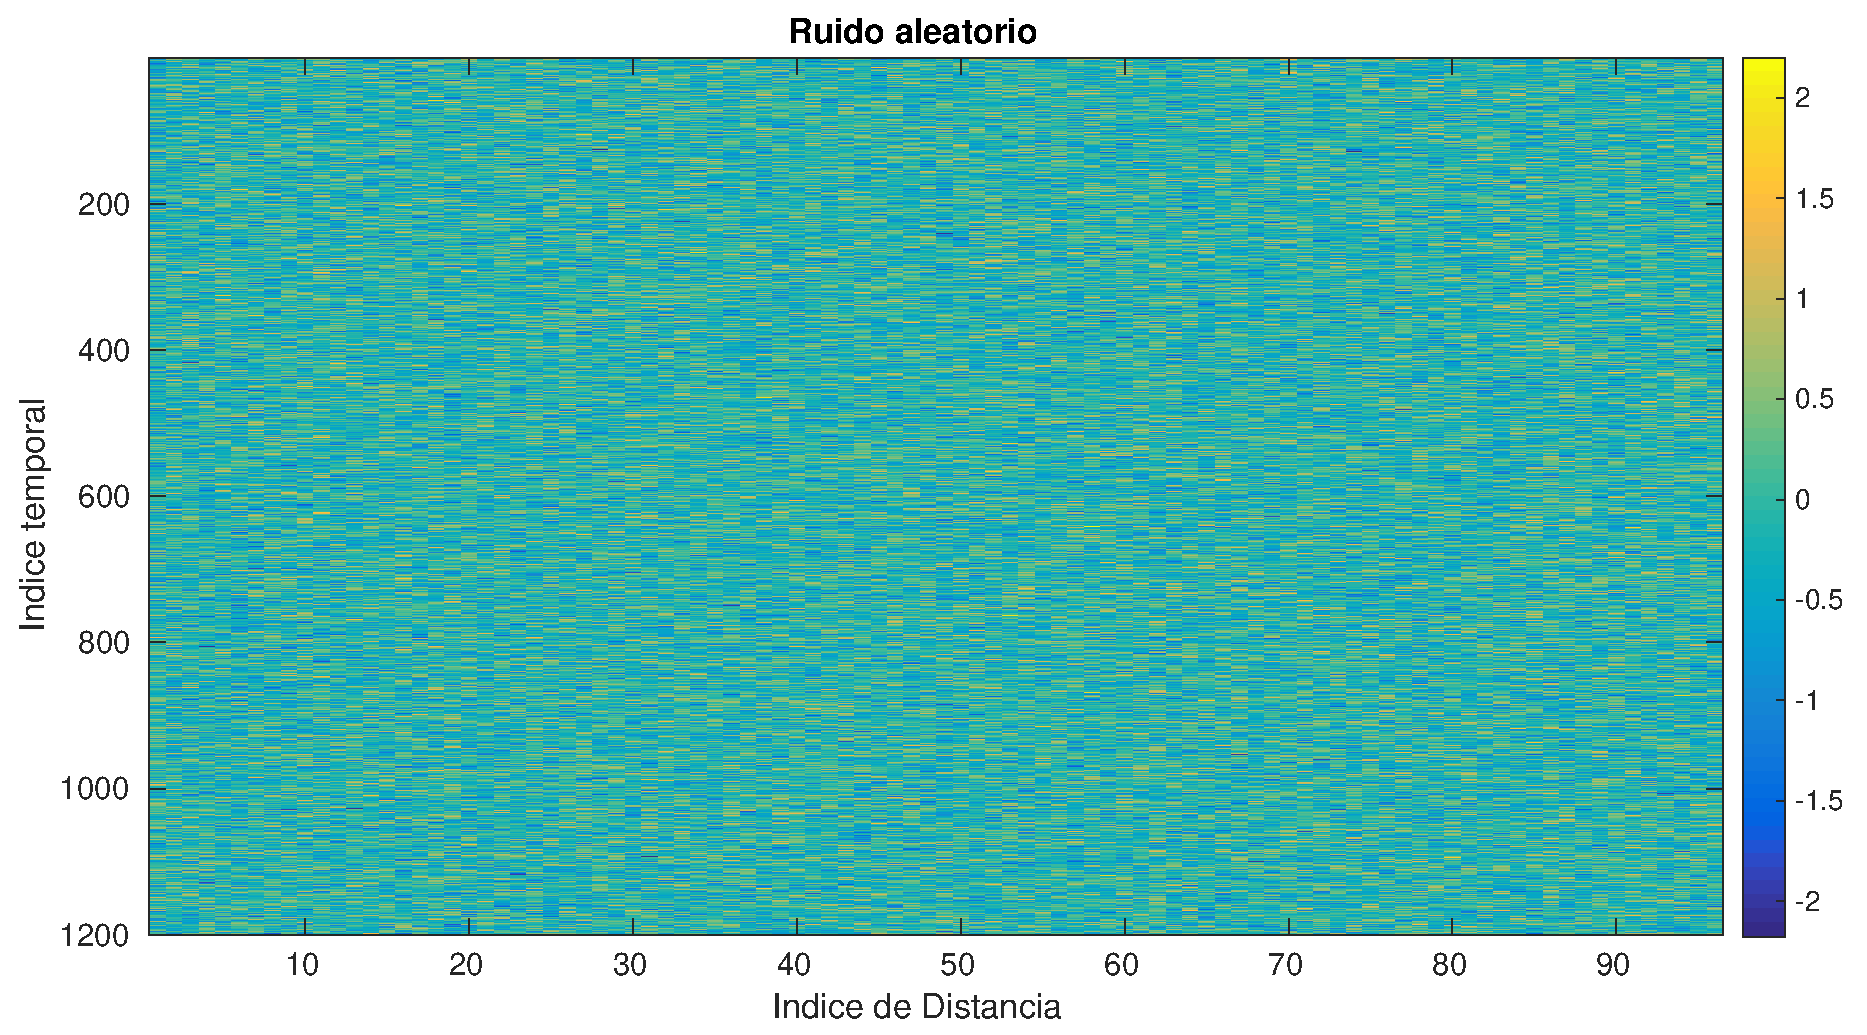
\includegraphics[totalheight=7.0cm]{figuras/cap3/ruido_aletorio.eps}
\caption{Ruído aleatório gerado no matlab}
\label{fig:ruido_aletorio}
\end{figure}

Nas seções sísmicas se precisa aplicar uma função de ganho devido à diminuição da amplitude com a distância-tempo, denominado de  espalhamento geométrico, divergência esférica, e às vezes atenuação tempo-distância. 
A função ganho empregada corresponde a uma amplificação do sinal no tempo para que se possa ver e interpretar a composição do sinal, que na sísmica é composto de eventos do tipo ruído, reflexões, refrações, múltiplas e difrações. 
Isto é, a correção de espalhamento geométrico por uma função ganho é aplicada para compensar o decaimento de energia da divergência da frente de onda em qualquer fase do processamento de uma seção sísmica. 
Ressalta-se que a aplicação de um ganho é uma operação destrutiva, ou não-destrutiva; o ganho aplicado é classificada como quase não-destrutivo devido ao ponto zero anulado.
A função ganho aplicada é dada por 

\begin{equation}
g(t)=t^{a}e^{-bt},
\label{eq:figura_ganho}
\end{equation}

onde os valores utilizados para os parâmetros foram $a=2$ e $b=0,5$.

\begin{figure}[H]
\centering
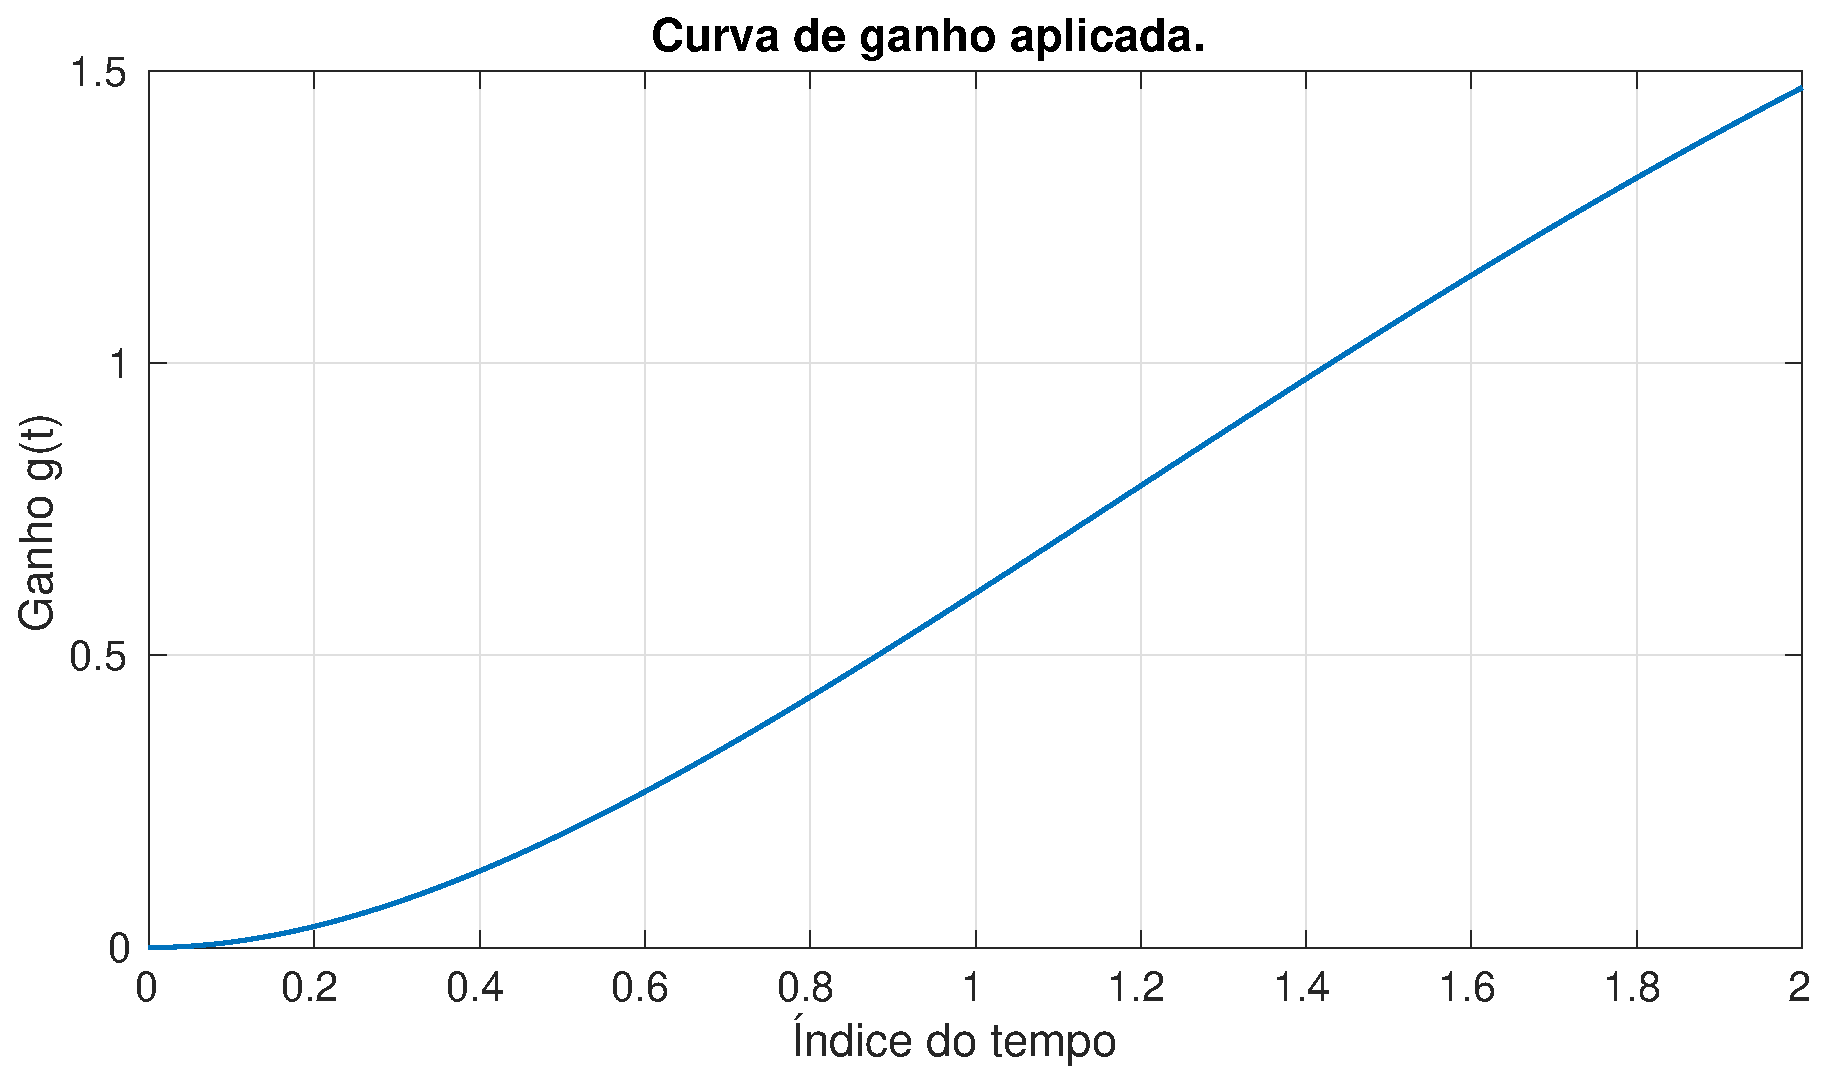
\includegraphics[totalheight=7.0cm]{figuras/cap3/figura_ganho.eps}
\caption{Função ganho empregada.}
\label{fig:figura_ganho}
\end{figure}

A figura \ref{fig:figura_ganho} mostra a variação do ganho, onde se observa que ela é crescente, mas com um intervalo de amplificação entre zero e $1,5$, que se apresenta de uma forma diferente, mas consistente no que se refere a colocar os valores num intervalo menor.  

Para que se possa realizar uma filtragem, a informação a ser recuperada deve ser separável do não-desejado, no domínio-f , ou no domínio-t.

A figura (\ref{fig:espc_tiro50}) mostra o espectro de amplitude da seção tiro 50 com ruído gerada a partir da figura (\ref{fig:tiro_50ruido}).

O termo filtro é reservado para a operação de multiplicação no domínio da frequência, e pode zerar a parte não desejada do espectro do sinal. Através da definição do espectro de amplitude e de fase podemos construir o operador $H(f)=A(f)e^{\theta(f)}$, que representa o filtro na frequência. Todo e qualquer processo de filtragem de um sinal pode ser representado na seguinte forma:

\begin{equation}
S_{H}(f)=G(f) H(f)
\label{eq:filtragem}
\end{equation}

Onde $S_{H}$ representa o sinal filtrado no domínio da frequência, $G(f)$ representa o sinal a ser filtrado e $H(f)$ o filtro a ser aplicado. Ou no domínio tempo na forma de convolução:

\begin{equation}
s_{h}(t)=s(t) \ast h(t)
\label{eq:filtragem_conv}
\end{equation}

As figuras (\ref{fig:espc_tiro50_c1}), (\ref{fig:espc_tiro50_c2}) e (\ref{fig:espc_tiro50_c3}) ilustram a geometria de passagem e rejeição de uma forma geral.

Após a filtragem da seção tiro 50 (ver figura \ref{fig:secao_filtrada}) nota-se que a maior parte da componente de ruído (informação não desejável) foi removida com a filtragem F-K. O corte no espectro de amplitude de maneira iterativa pelo matlab permite maior precisão na eliminação do ruído. Comparando a figura (\ref{fig:secao_filtrada}) com (\ref{fig:tiro_50ruido}), respectivamente a seção tiro 50 filtrada sem ganho e seção tiro 50 com ruído.

Em seguida a figura (\ref{fig:secao_filtrada_gain}) mostra a atuação do ganho na seção tiro 50 filtrada, o ganho aumenta com o tempo ou seja não apenas os eventos desejavéis são amplificados como também a componente de ruído. Comparando as duas figuras (\ref{fig:secao_filtrada_gain}) com (\ref{fig:tiro_50ruido_gain}) onde respectivamente representam a seção tiro 50 filtrada com ganho e seção tiro 50 com ruído e ganho. 

\begin{landscape}
\begin{figure}[H]
\centering
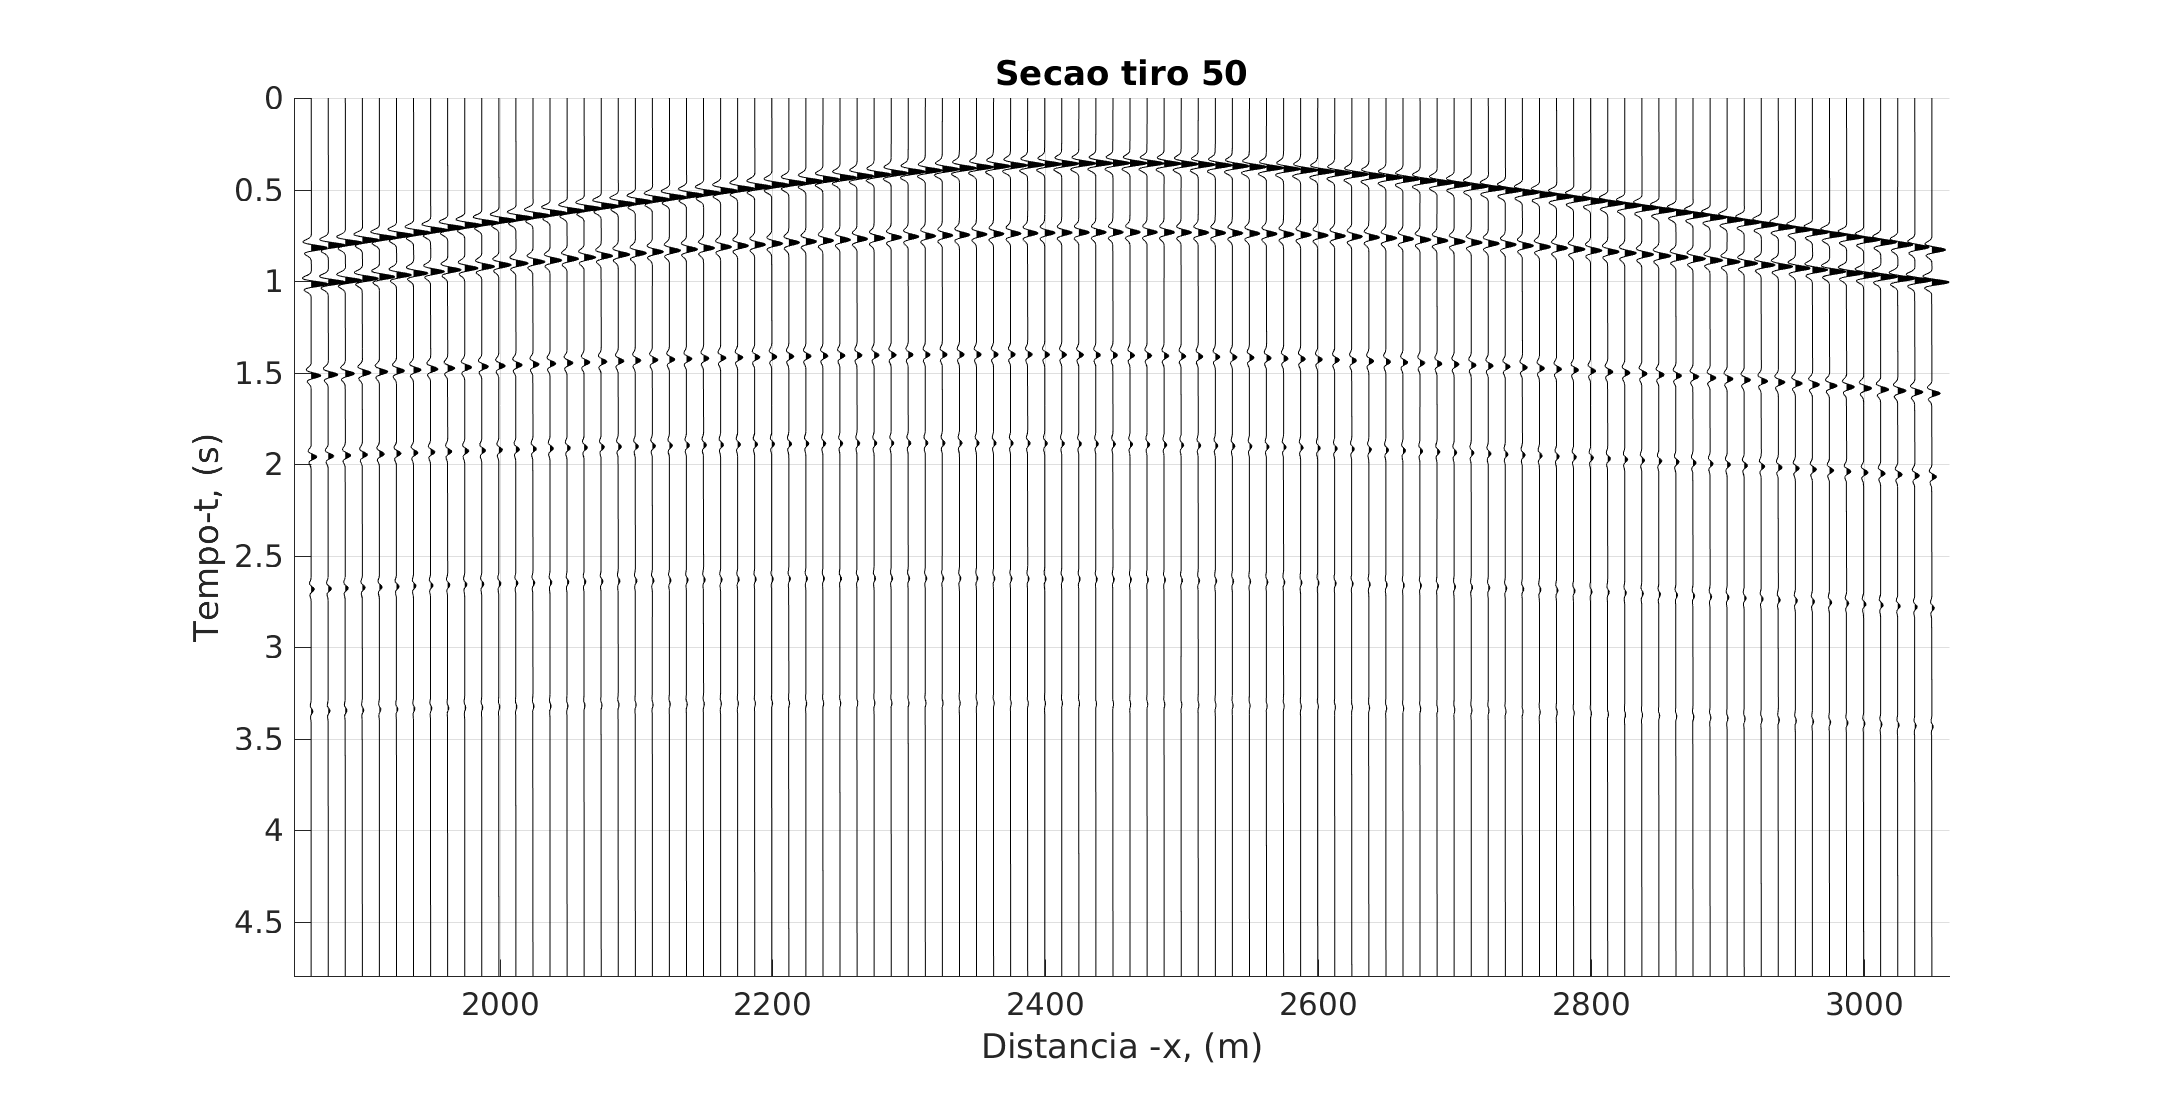
\includegraphics[totalheight=14cm]{figuras/cap3/secao_tiro50.eps}
\caption{Seção tiro 50 sem ganho do modelo sintético, figura (\ref{fig:vagarosidade})}
\label{fig:tiro_50}
\end{figure}
\end{landscape}

\begin{landscape}
\begin{figure}[H]
\centering
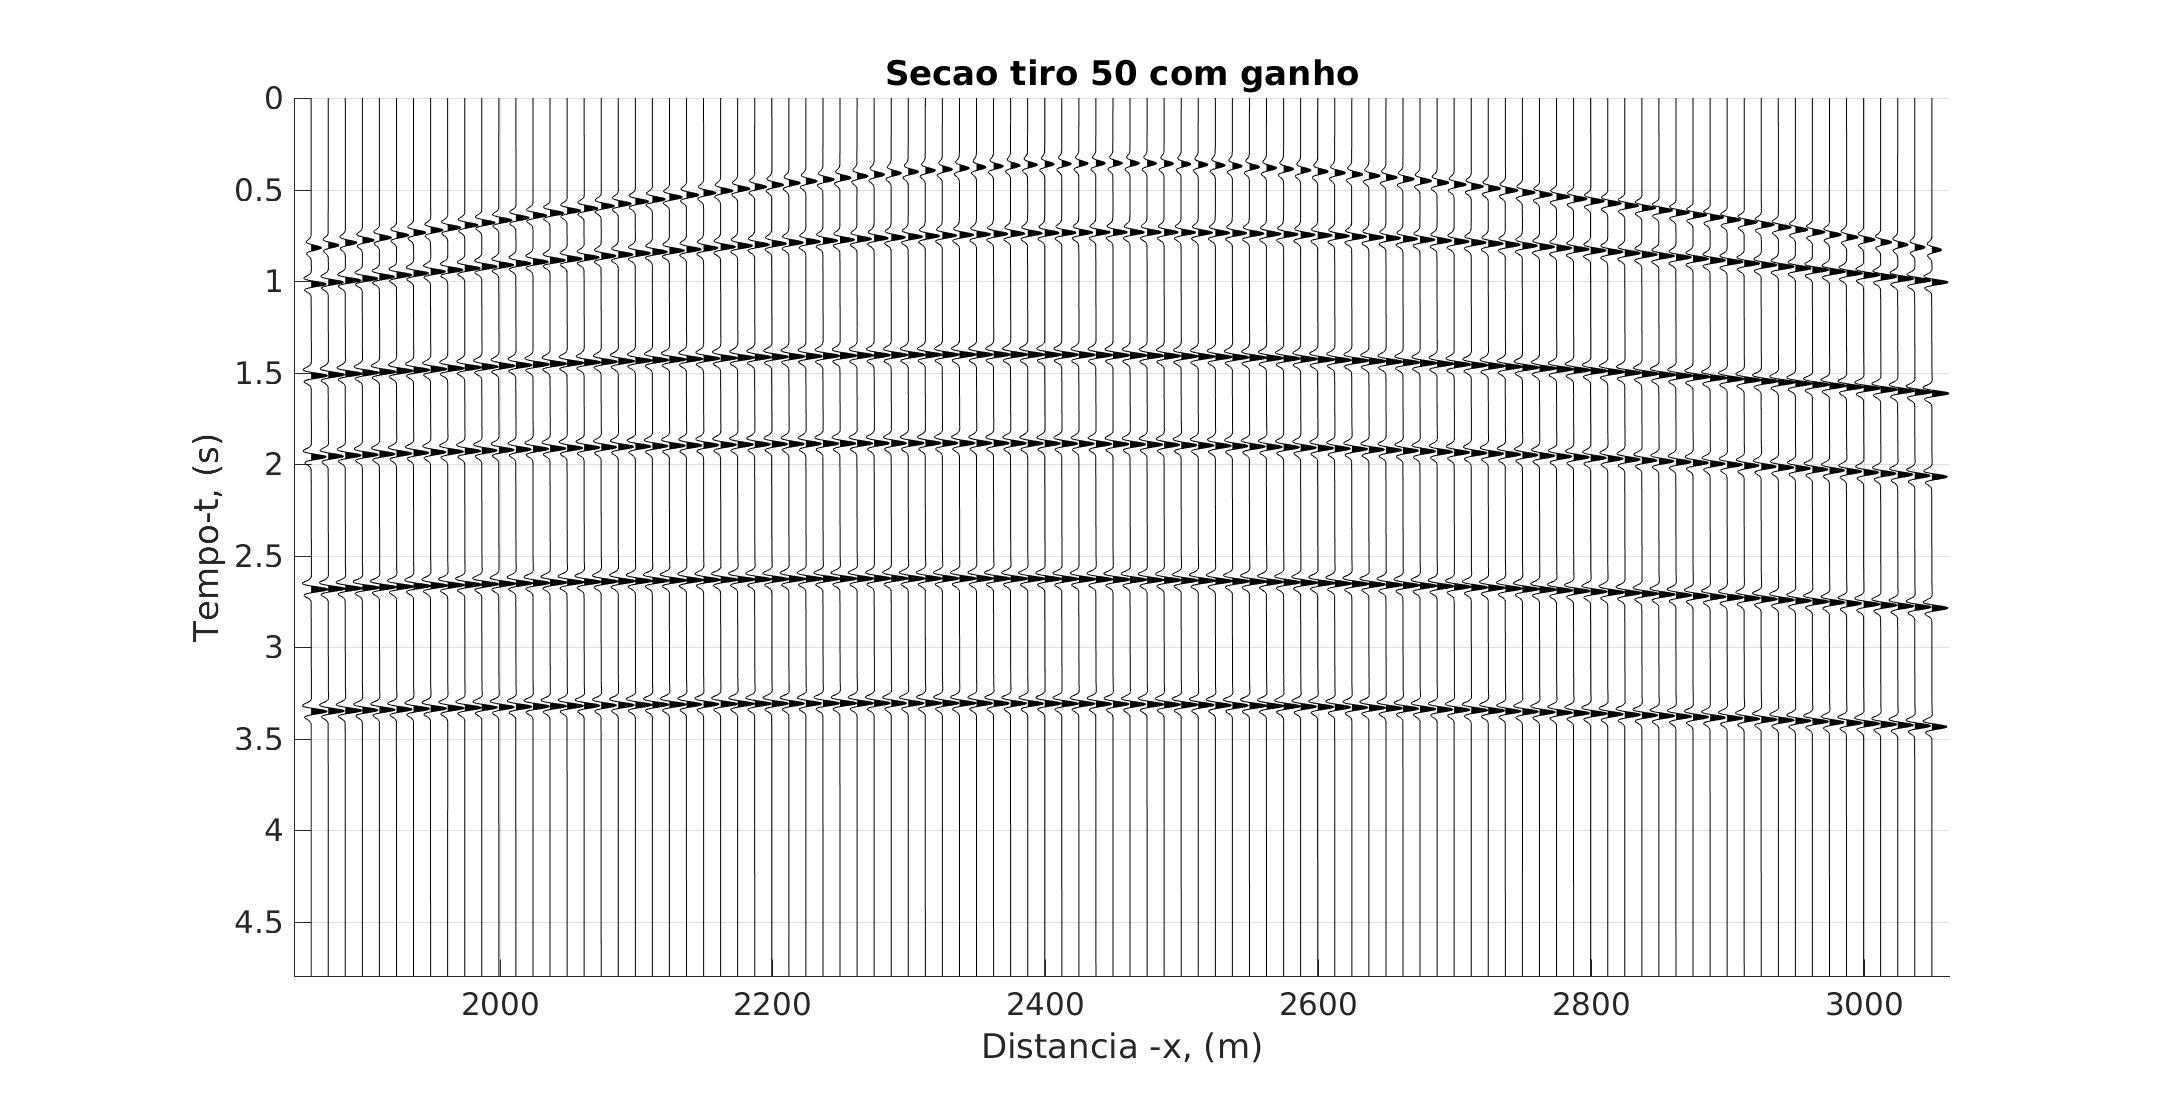
\includegraphics[totalheight=14cm]{figuras/cap3/secao_tiro50_ganho.eps}
\caption{Seção tiro 50 com ganho, os eventos com maior tempo foram realçados.}
\label{fig:tiro_50gain}
\end{figure}
\end{landscape}

\begin{landscape}
\begin{figure}[H]
\centering
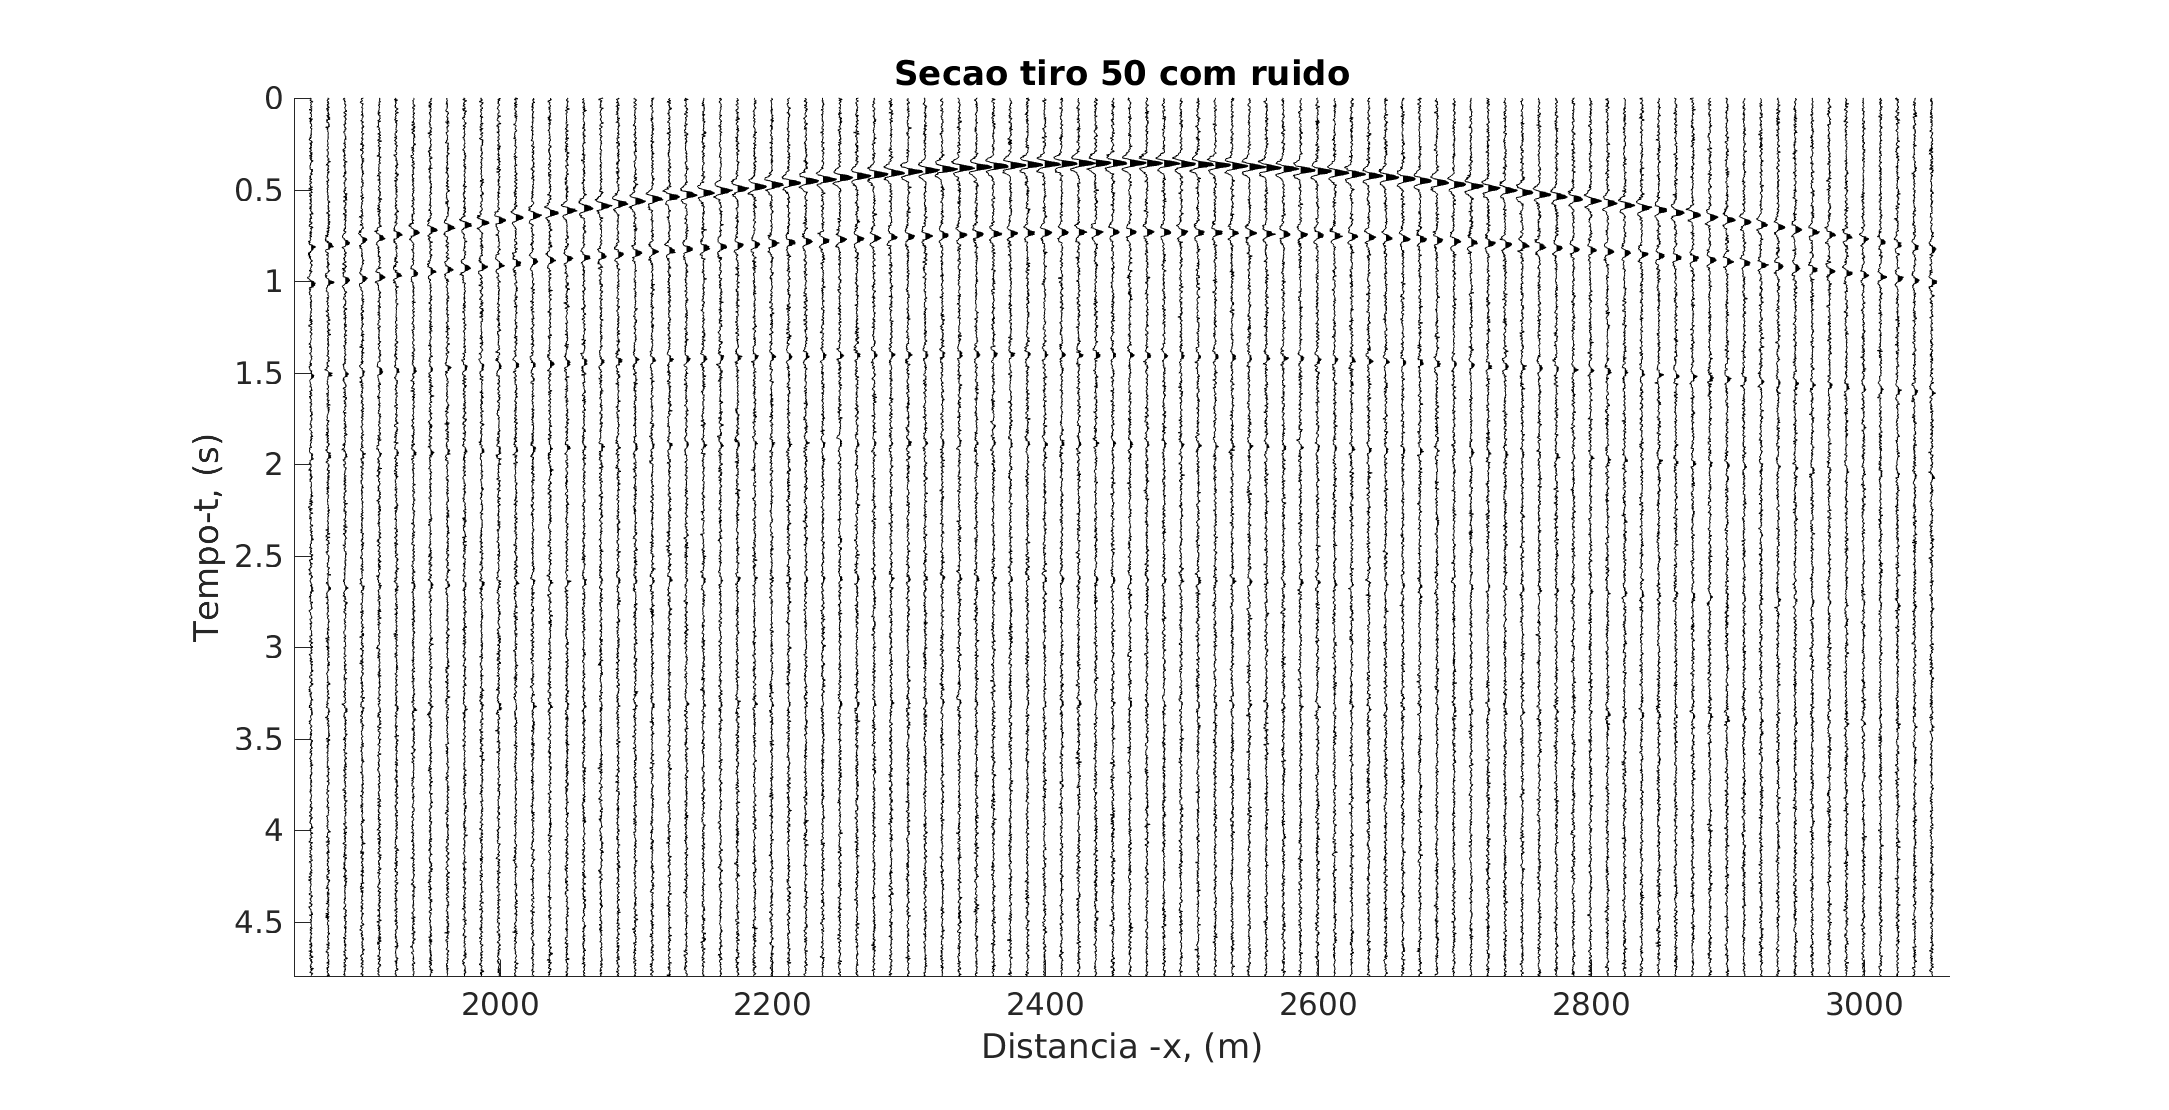
\includegraphics[totalheight=14cm]{figuras/cap3/secao_tiro50_ruido.eps}
\caption{Seção tiro 50 com ruido aleatório, o ruído foi gerado no matlab e somado a seção tiro 50.}
\label{fig:tiro_50ruido}
\end{figure}
\end{landscape}

\begin{landscape}
\begin{figure}[H]
\centering
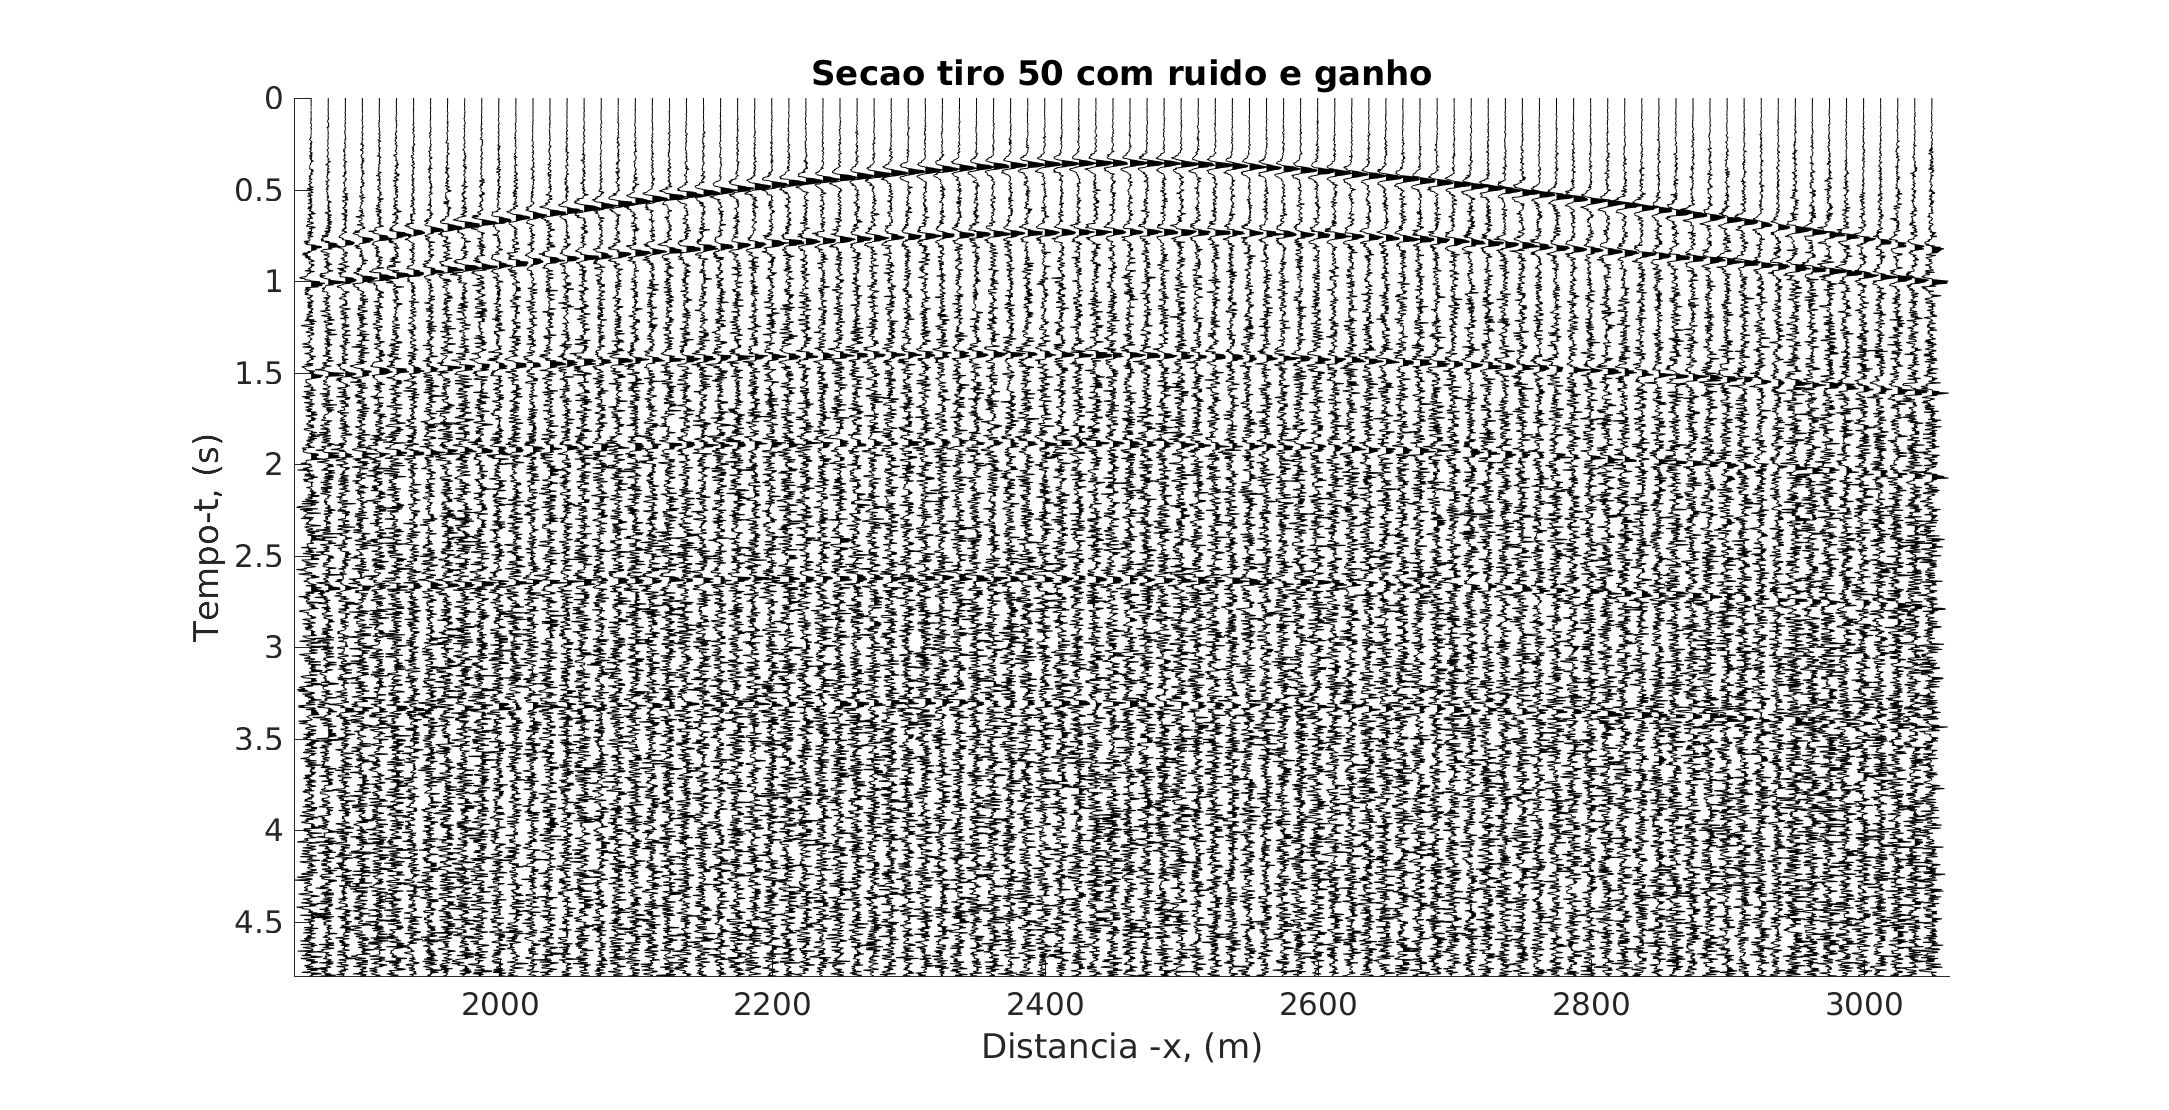
\includegraphics[totalheight=14cm]{figuras/cap3/secao_tiro50_ruido_gain.eps}
\caption{Seção tiro 50 com ruido e ganho, a informação e o ruído foram amplificados, os eventos de maior tempo foram ``mascarados'' com a amplificação da função ganho.}
\label{fig:tiro_50ruido_gain}
\end{figure}
\end{landscape}

\begin{landscape}
\begin{figure}[H]
\centering
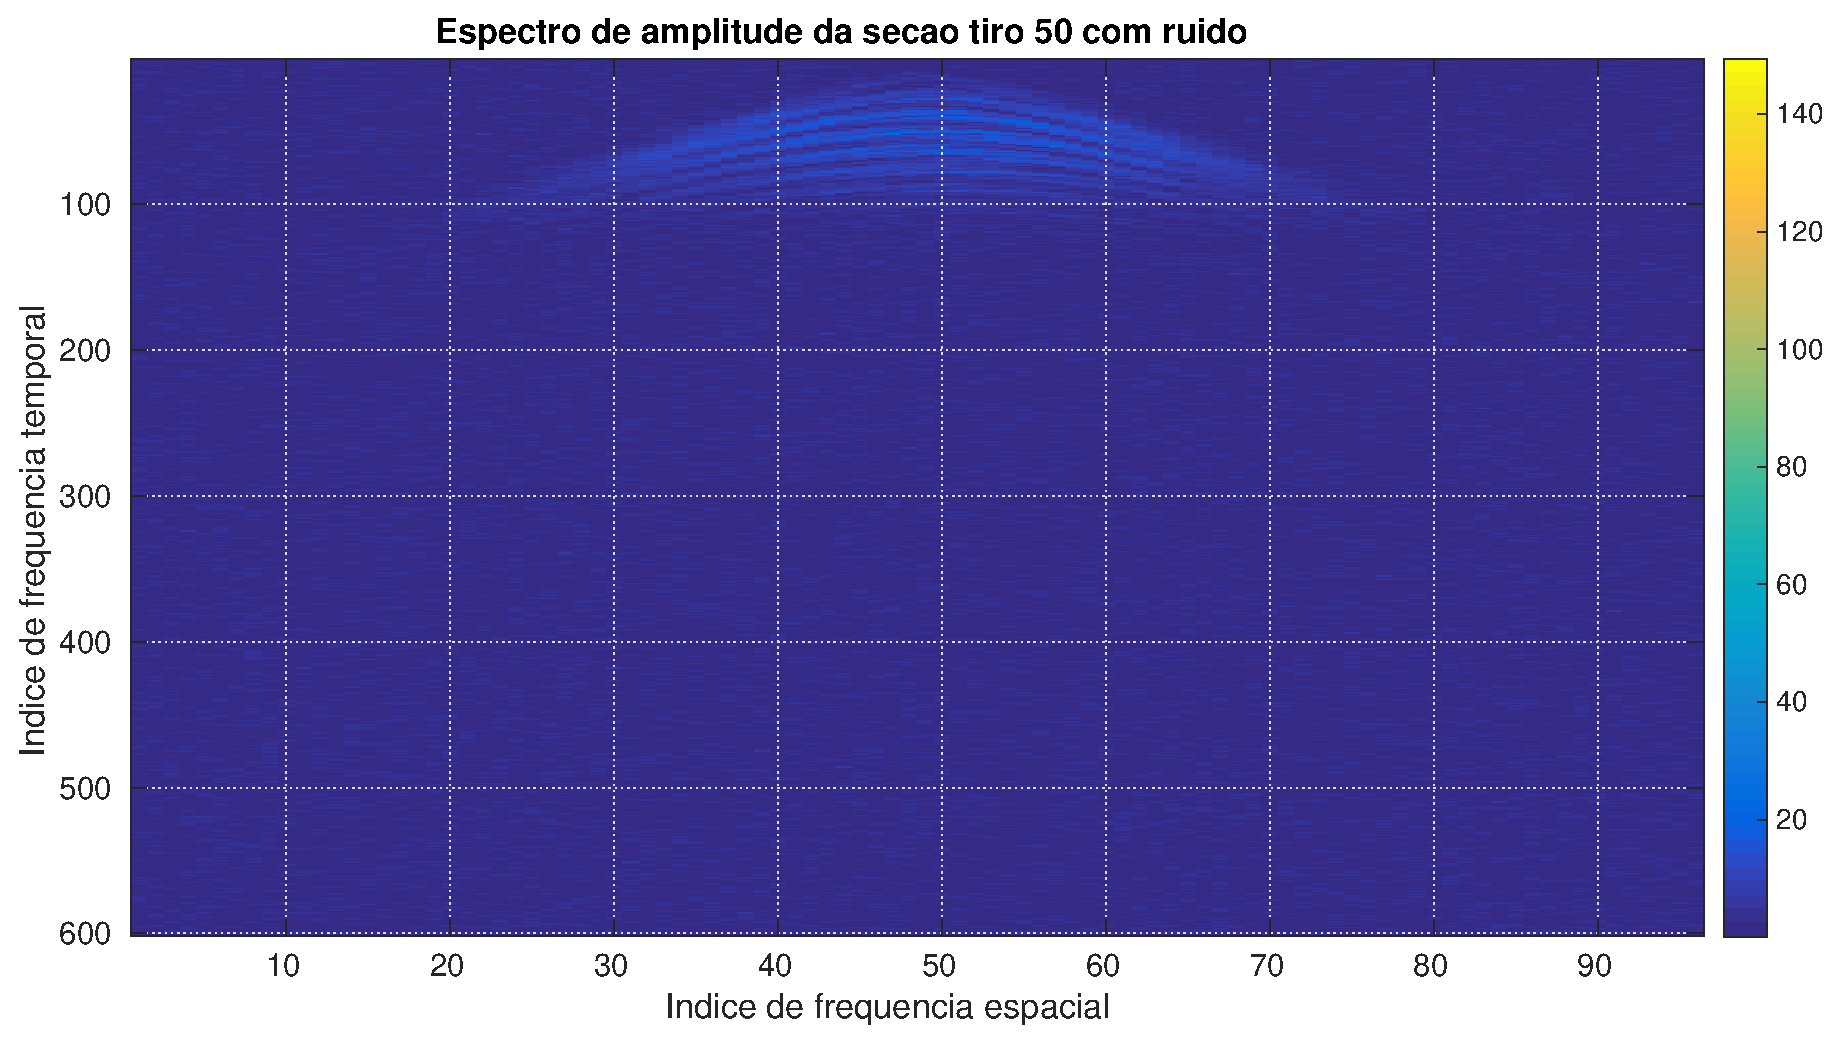
\includegraphics[totalheight=14cm]{figuras/cap3/espc_tiro50.eps}
\caption{Espectro da seção tiro 50 com ruído, este espectro não apresenta falseamento de informação tanto em $f_t$ (frequência temporal) quanto em $f_k$ (frequência espacial).}
\label{fig:espc_tiro50}
\end{figure}
\end{landscape}

\begin{landscape}
\begin{figure}[H]
\centering
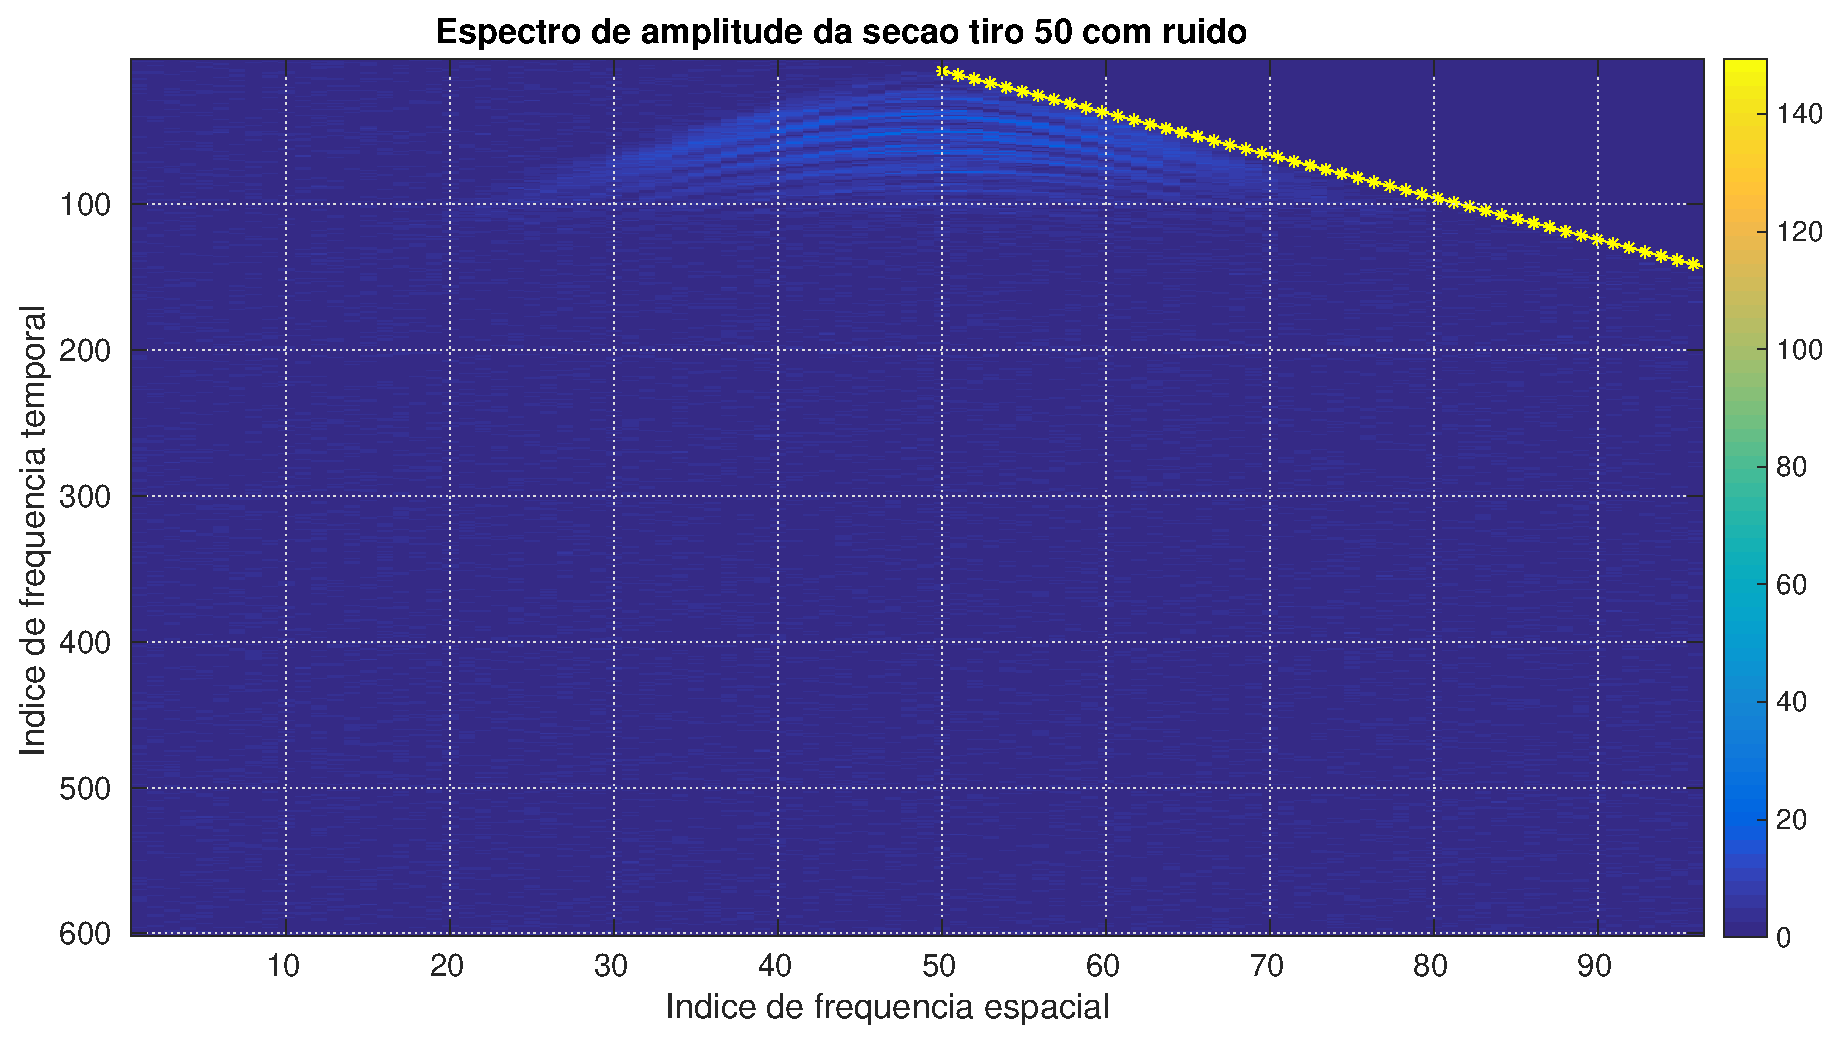
\includegraphics[totalheight=14cm]{figuras/cap3/espc_tiro50_c1.eps}
\caption{Seção tiro 50 com ruído após o primeiro corte (linha amarela) no espectro de amplitude.}
\label{fig:espc_tiro50_c1}
\end{figure}
\end{landscape}

\begin{landscape}
\begin{figure}[H]
\centering
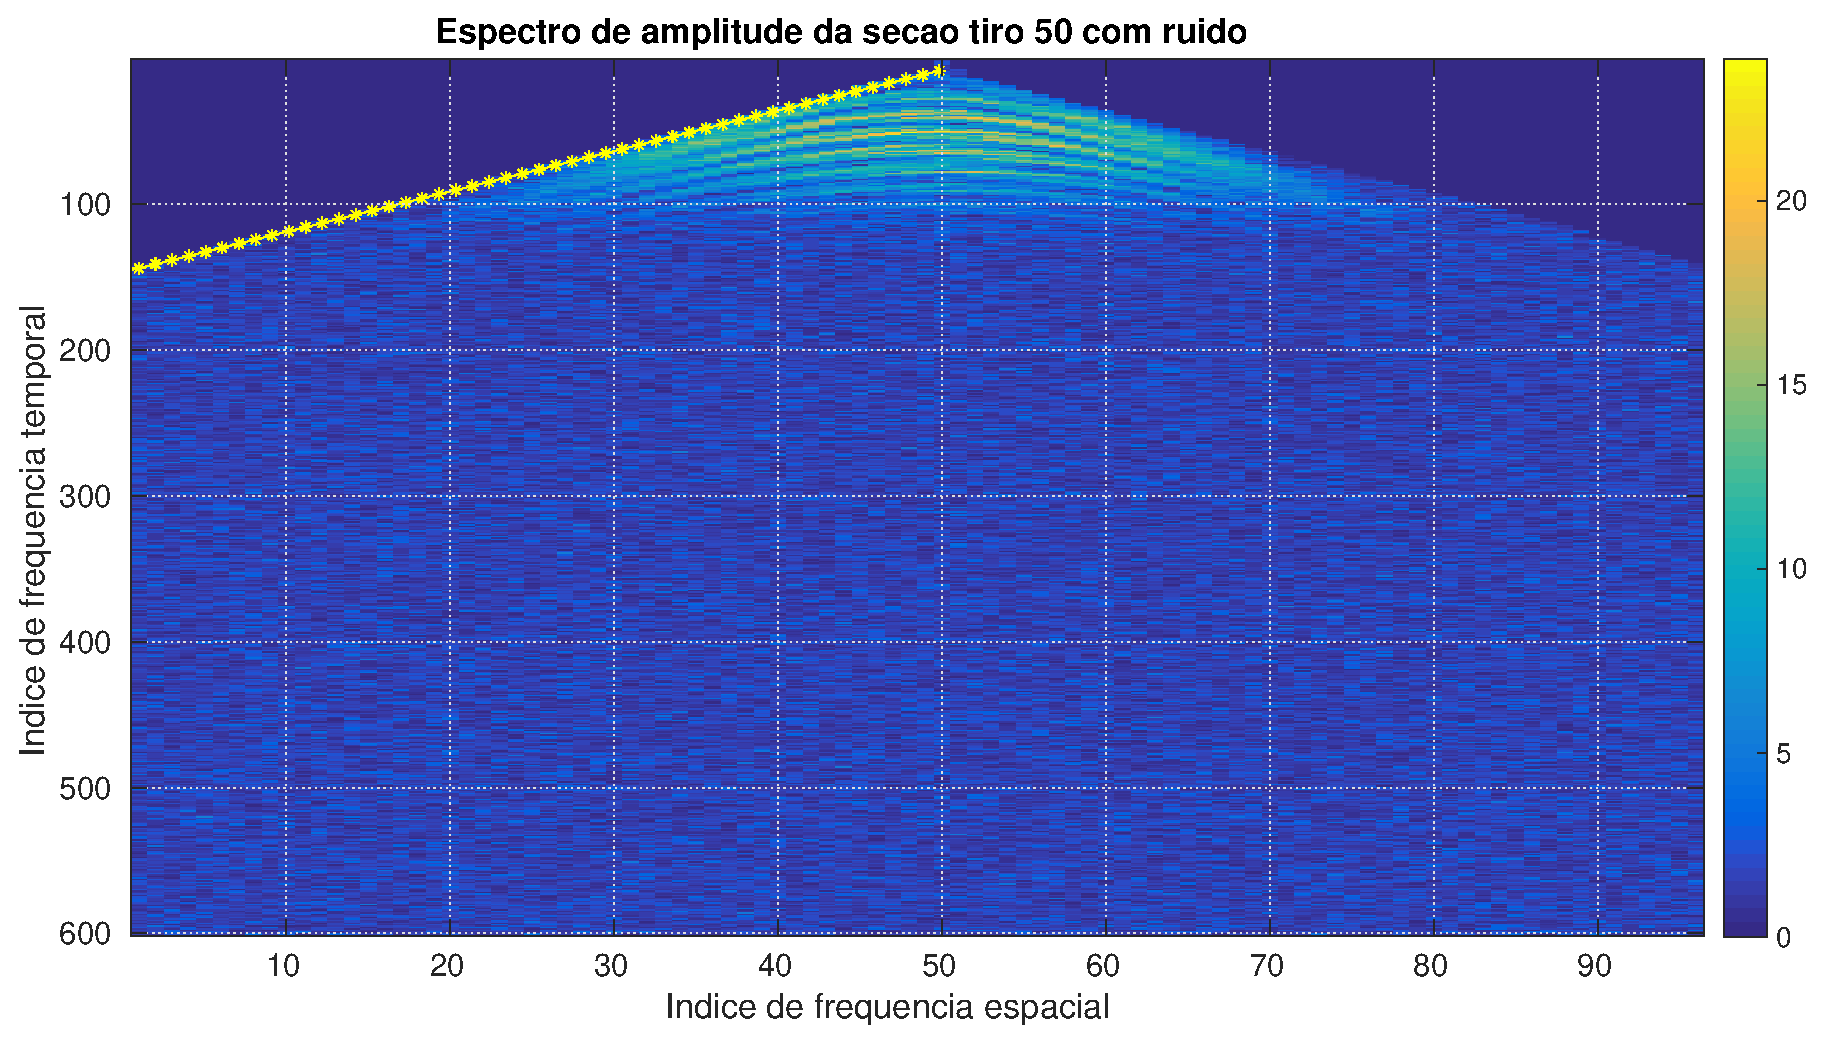
\includegraphics[totalheight=14cm]{figuras/cap3/espc_tiro50_c2.eps}
\caption{Seção tiro 50 com ruído após o segundo corte (linha amarela) no espectro de amplitude.}
\label{fig:espc_tiro50_c2}
\end{figure}
\end{landscape}

\begin{landscape}
\begin{figure}[H]
\centering
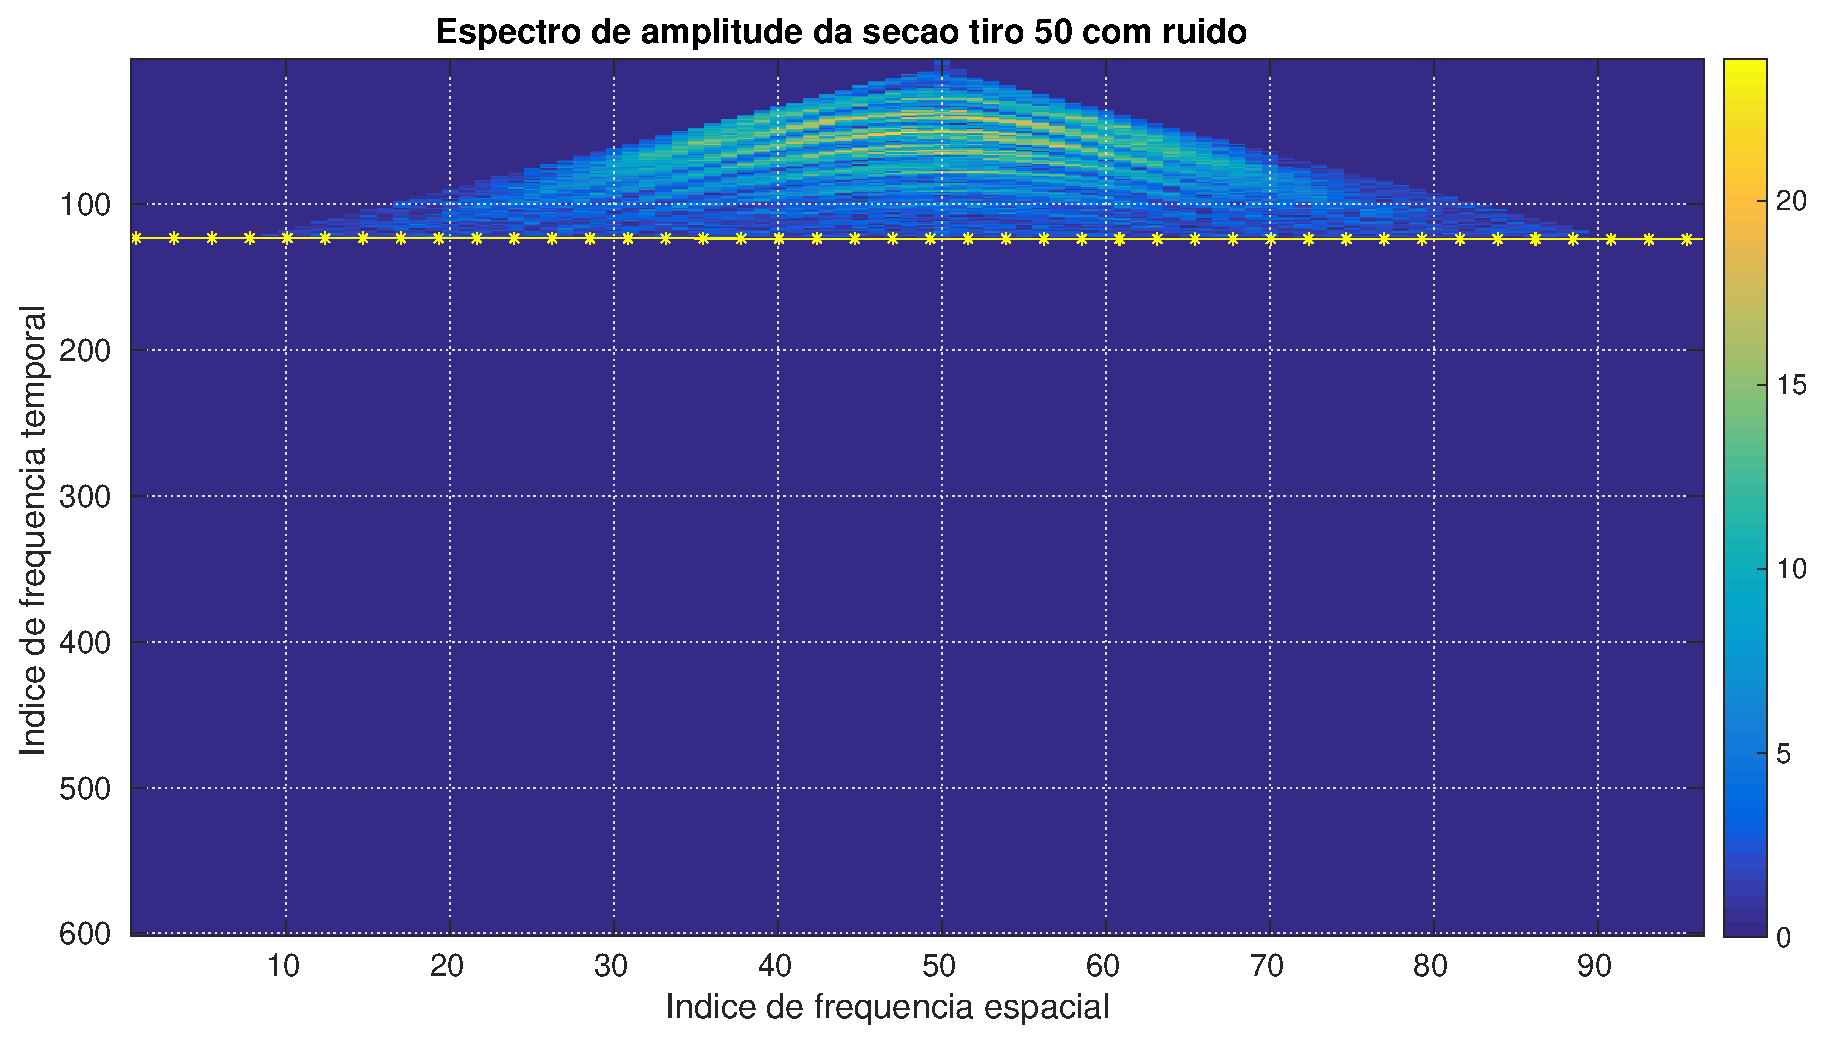
\includegraphics[totalheight=14cm]{figuras/cap3/espc_tiro50_c3.eps}
\caption{Seção tiro 50 com ruído após o terceiro corte (linha amarela) no espectro de amplitude.}
\label{fig:espc_tiro50_c3}
\end{figure}
\end{landscape}

\begin{landscape}
\begin{figure}[H]
\centering
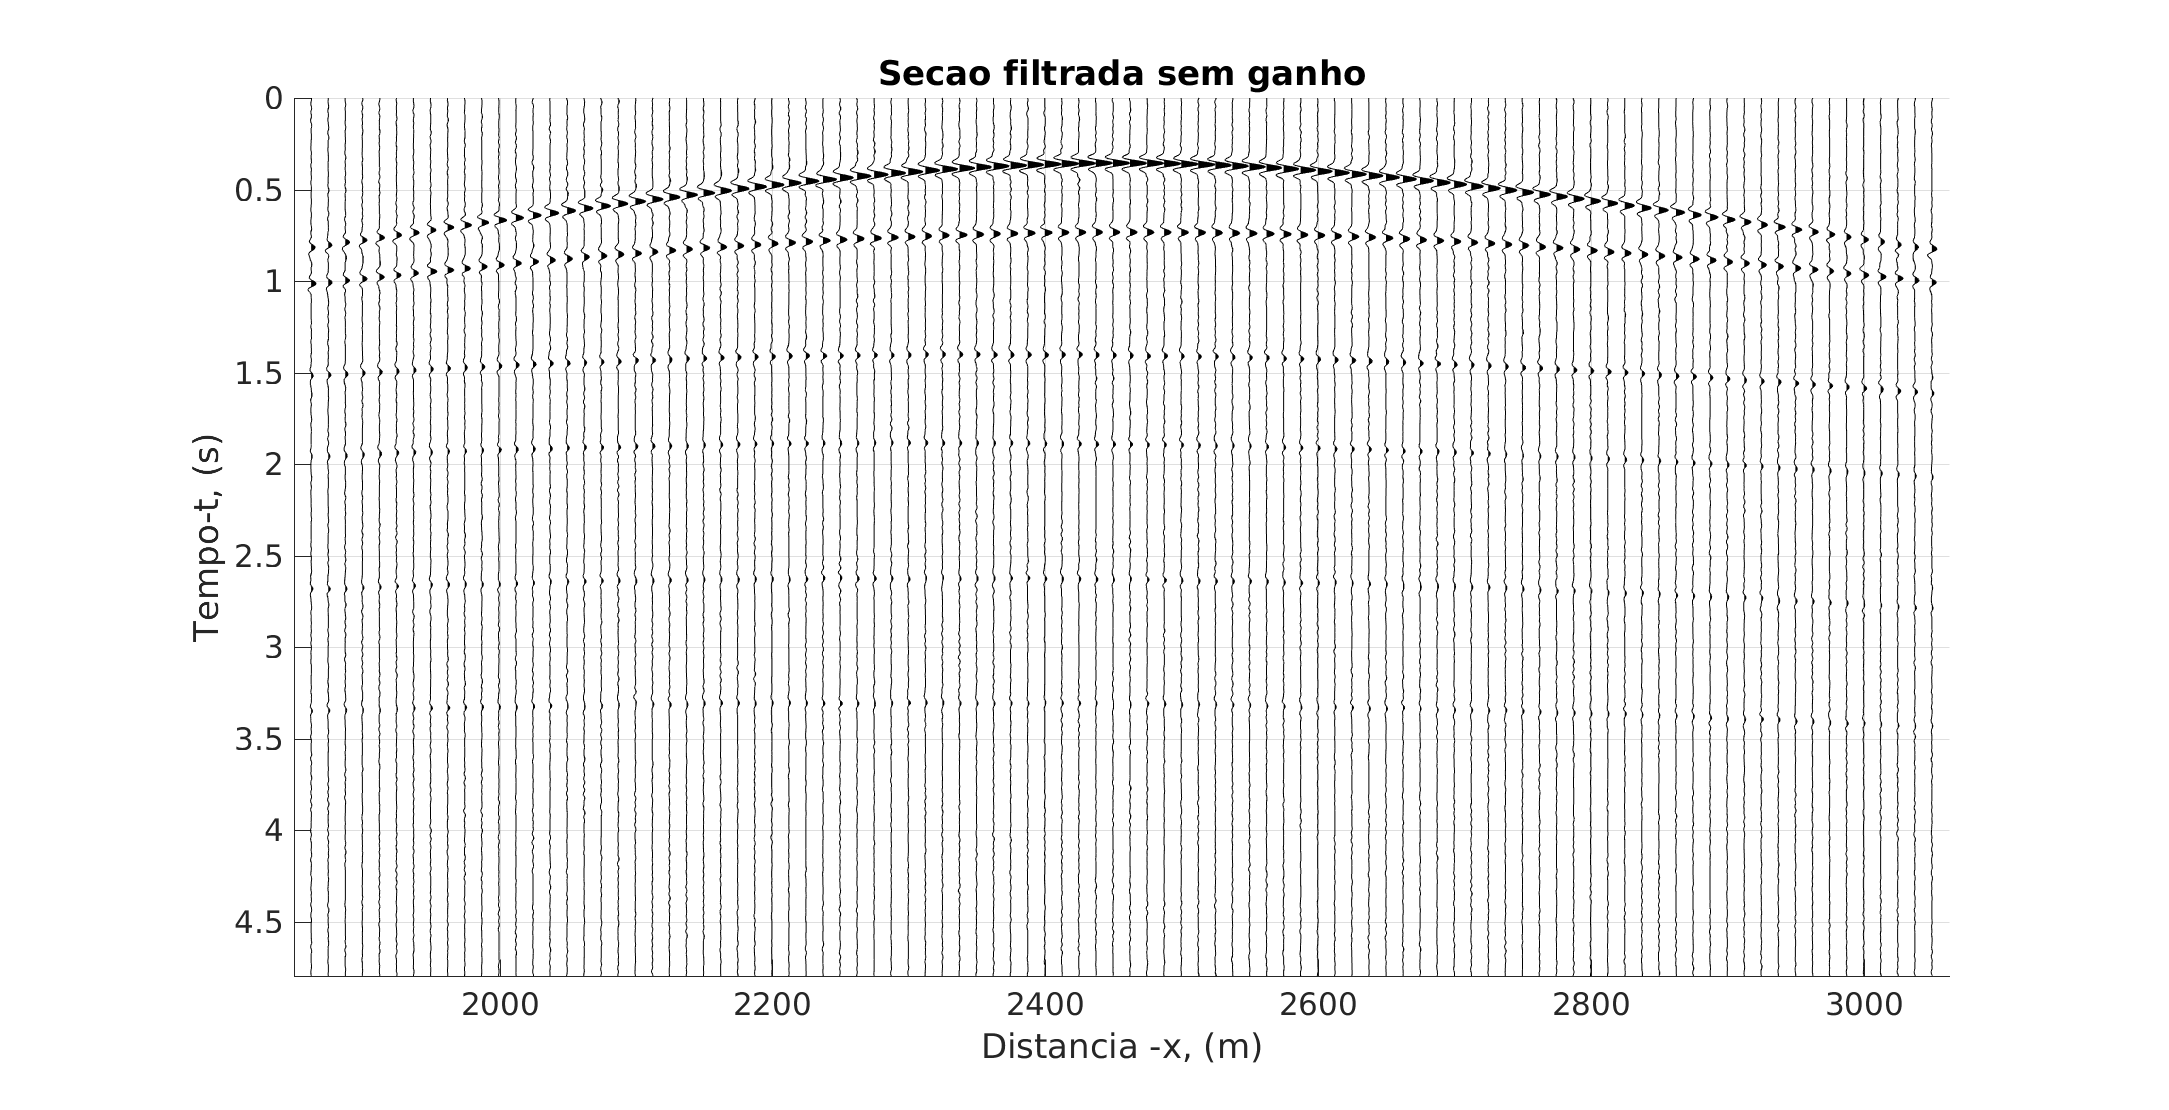
\includegraphics[totalheight=14cm]{figuras/cap3/secao_filtrada.eps}
\caption{Seção tiro 50 filtrada do ruído sem ganho, comparando a figura (\ref{fig:tiro_50ruido}) nota-se que a componente do ruído foi em grande parte removida após a filtragem F-K.}
\label{fig:secao_filtrada}
\end{figure}
\end{landscape}

\begin{landscape}
\begin{figure}[H]
\centering
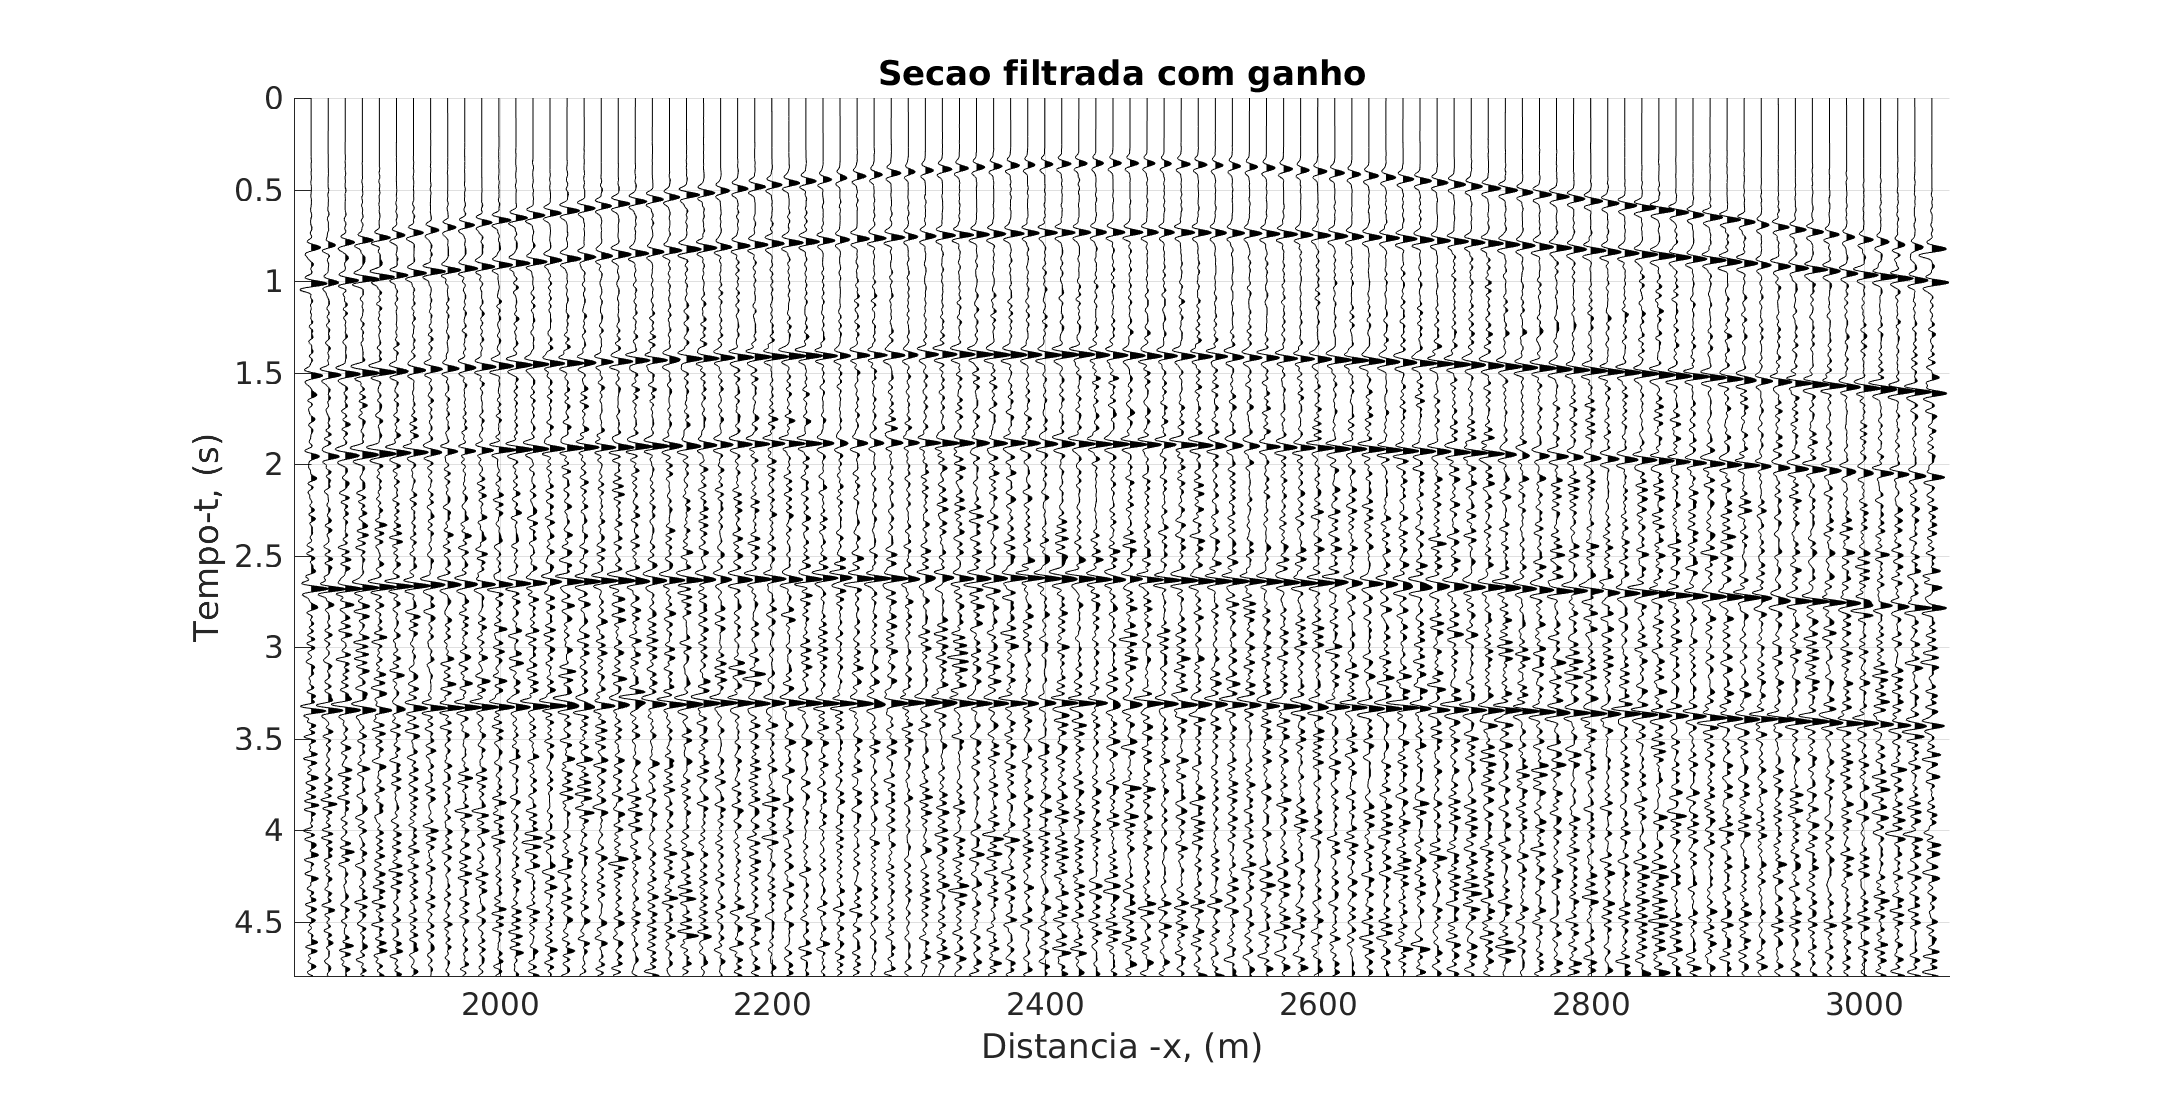
\includegraphics[totalheight=14cm]{figuras/cap3/secao_filtrada_gain.eps}
\caption{Seção tiro 50 filtrada do ruído com ganho, comparando a figura (\ref{fig:tiro_50ruido_gain}) nota-se que os eventos com maior tempo foram recuperados. O ganho amplificou tanto a informação de interesse (eventos) quanto o ruído.}
\label{fig:secao_filtrada_gain}
\end{figure}
\end{landscape}